\chapter{Finite difference time domain}

Finite difference methods are a powerful class of computational tools that seek to solve Maxwell's equations over a given simulation space. In the time domain, the electromagnetic fields are obtained by discretising both time and space over a structured space known as the Yee grid, and approximating the fields by finite differences. A finite difference is simply an approximate solution to a differential equation - consider the first derivative of some function $f$,

\begin{equation}
f'(x) = \lim_{h \rightarrow 0} \dfrac{f(a+h) - f(a)}{h}.
\end{equation}

A reasonable approximation for this, assuming some small value of $h$ is simply

\begin{equation}
f'(x) = \dfrac{f(a+h) - f(a)}{h}.
\end{equation}

In principle, this can be applied to solving Maxwell's equation

A major weakness of the \textit{FDTD} method, and indeed, any method that implements materials on a Yee grid is the way in which it handles boundaries that are not aligned to the grid.

 
\section{Formulation of the FDTD method}

We begin with the fully vectorised Maxwell equations in $3D$,

\begin{align}
\partial_y E_z - \partial_z E_y &= \mu_{xx} H_x \\
\partial_z E_x - \partial_x E_z &= \mu_{yy} H_y \\
\partial_x E_y - \partial_y E_x &= \mu_{zz} H_z 
\end{align}

for the $\bm{H}$ field, and 

\begin{align}
\partial_y H_z - \partial_z H_y &= \mu_{xx} E_x \\
\partial_y H_z - \partial_z H_y &= \mu_{xx} E_y \\
\partial_y H_z - \partial_z H_y &= \mu_{xx} E_z 
\end{align}

for the $\bm{E}$ field, where we have adopted the notation $\frac{\partial}{\partial i} = \partial_i$ for brevity. Likewise, the diagonally anisotropic material tensors for the permittivity and permeability are represented through $\epsilon$ and $\mu$ respectively. Throughout this thesis, we will assume anisotropy of the material, that is, 

To eliminate the high frequency components that would otherwise emerge due to the instantaneous `switching-on' of the field source, we construct a ramp function that linearly increases the amplitude of the wave to a maximum. 

The difficulty in adapting finite difference methods in simulating \textit{active} nanophotonic materials is that there is no pre-existing framework for modifying the simulation while it is running (i.e., designing a moving structure). The effects of motion can be simulated by using a separate source to change the refractive index of the material, but this method introduces its own problems - the pump source can and in most cases will interfere with the original source. The most obvious way to bypass these problems is to directly update the permittivity of the simulation at each time-step. Although this requires having to recalculate the update coefficients of the simulation every time-step, it is by far the easiest method to implement. 

\subsection{Dispersion and stability}
\textit{FDTD} generally provides a good approximation to the real physical behaviour of fields. However, taking finite differences of normally continuous functions naturally introduces an error. For instance, the group velocity of some wave propagating in the Yee grid will in general differ from $c$. This discrepancy depends on several factors including the spatial grid size, direction of propagation, and even the frequency of incident light. Such errors are known as \textit{dispersion}.

FDTD samples the electromagnetic field at points that are discrete in both time and space. The choice of these steps is thus important for maintaining the \textit{stability} of the solution. 

\subsection{Perfectly matched layer}
The Perfectly Matched Layer (PML) is an artificial medium that is developed to absorb EM waves incident from any direction with virtually no reflection. Since EM waves incident on PML do not reflect backwards, a simulation domain surrounded by PML effectively represents an open space, and is used commonly in finite difference methods to simulate spatially unbounded systems.

\subsection{Modal source}
To excite a mode in a wave guide it is insufficient to merely place a point sinusoidal source at some arbitrary location. Even with a priori knowledge of the mode wave vector $k$ and frequency $\omega$, the source is more likely to excite several modes within a range of frequencies. The transfer matrix formalism for photonic transitions require the input wave to be in an already exact mode. If there are multiple modes passing through a modulated region, each will be transitioned up a level of the band structure in turn.
Typically, the method used to excite modes in \textit{FDTD} is to place a \textit{gaussian} source of the form

\begin{equation}
f_{g} = e
\end{equation}

Such a Gaussian source possesses an effectively infinite number of frequencies, and is thus capable of exciting any number of modes around the frequency width chosen. 

However, photonic transitions require that a perfect mode $\ket{1}$ is actuated in the waveguide at the beginning of the simulation. To achieve this, the previously written wave guide band solver can be adjusted to return a field amplitude profile in the exact shape of the required mode. This means a source can be excited simply by choosing a line input, passing the parameters of the wave guide to the band solver, and obtaining a mode at a pre-defined frequency (or equivalently, wave vector). This is demonstrated in figure \ref{fig:modes}, where the output of the mode solver is shown for the first fundamental $\ket{1}$ and second $\ket{2}$ TE modes for a waveguide of width $1.1 \mu m$ and permittivity $10$. Directly writing these modes into the curl update equations for $E_x$ and $H_y$ allow for one-way propagation. This is useful, as it means that the simulation space has effectively been split into two regions: one containing the reflected wave, and another containing the incident wave. This method is employed for the remainder of this thesis. In figure \ref{fig:3dmode} a $3D$ representation of the first mode $\ket{1}$ is shown. 

\begin{figure}[t]
\centering
\setlength{\figH}{0.5\textwidth}
\setlength{\figW}{0.5\textwidth}
\begin{subfigure}[t]{0.5\textwidth}
	% This file was created by matlab2tikz.
%
%The latest updates can be retrieved from
%  http://www.mathworks.com/matlabcentral/fileexchange/22022-matlab2tikz-matlab2tikz
%where you can also make suggestions and rate matlab2tikz.
%
\definecolor{mycolor1}{rgb}{0.00000,0.44600,0.74200}%
\definecolor{mycolor2}{rgb}{0.46667,0.67451,0.18824}%
%
\begin{tikzpicture}

\begin{axis}[%
width=0.75\figW,
height=0.4\figH,
at={(0\figW,0.6\figH)},
scale only axis,
xlabel={$\text{y (}\mu\text{m)}$},
ylabel={$E_z$ ($V/\mu m$)},
xmin=-1,
xmax=1,
ymin=-1,
ymax=1,
%%
axis background/.style={fill=white}
]
\addplot [color=mycolor1, forget plot]
  table[row sep=crcr]{%
-0.55	0.162969143188896\\
-0.539	0.190666665332457\\
-0.528	0.218213195384856\\
-0.517	0.245586918792565\\
-0.506	0.272766157850501\\
-0.495	0.29972938886896\\
-0.484	0.326455259218582\\
-0.473	0.352922604239856\\
-0.462	0.379110464003759\\
-0.451	0.404998099910273\\
-0.44	0.430565011111631\\
-0.429	0.455790950747268\\
-0.418	0.480655941977656\\
-0.407	0.505140293804285\\
-0.396	0.529224616663298\\
-0.385	0.552889837780404\\
-0.374	0.576117216274925\\
-0.363	0.598888358001009\\
-0.352	0.621185230114262\\
-0.341	0.64299017535225\\
-0.33	0.664285926017585\\
-0.319	0.685055617652497\\
-0.308	0.705282802394075\\
-0.297	0.724951461999608\\
-0.286	0.744046020531692\\
-0.275	0.762551356693074\\
-0.264	0.78045281580146\\
-0.253	0.797736221394798\\
-0.242	0.814387886457854\\
-0.231	0.830394624261188\\
-0.22	0.845743758803939\\
-0.209	0.860423134852165\\
-0.198	0.874421127564773\\
-0.187	0.88772665169942\\
-0.176	0.900329170391103\\
-0.165	0.912218703496477\\
-0.154	0.923385835497295\\
-0.143	0.933821722956714\\
-0.132	0.943518101522557\\
-0.121	0.952467292471992\\
-0.11	0.96066220879244\\
-0.099	0.968096360793897\\
-0.088	0.974763861248226\\
-0.077	0.980659430051355\\
-0.066	0.985778398404671\\
-0.055	0.990116712512328\\
-0.044	0.993670936791508\\
-0.033	0.99643825659312\\
-0.022	0.998416480430764\\
-0.011	0.99960404171621\\
0	1\\
0.011	0.99960404171621\\
0.022	0.998416480430764\\
0.033	0.99643825659312\\
0.044	0.993670936791508\\
0.055	0.990116712512328\\
0.0660000000000001	0.985778398404671\\
0.077	0.980659430051355\\
0.088	0.974763861248226\\
0.099	0.968096360793897\\
0.11	0.96066220879244\\
0.121	0.952467292471992\\
0.132	0.943518101522557\\
0.143	0.933821722956714\\
0.154	0.923385835497295\\
0.165	0.912218703496477\\
0.176	0.900329170391102\\
0.187	0.88772665169942\\
0.198	0.874421127564773\\
0.209	0.860423134852166\\
0.22	0.845743758803939\\
0.231	0.830394624261188\\
0.242	0.814387886457854\\
0.253	0.797736221394798\\
0.264	0.78045281580146\\
0.275	0.762551356693074\\
0.286	0.744046020531692\\
0.297	0.724951461999608\\
0.308	0.705282802394075\\
0.319	0.685055617652497\\
0.33	0.664285926017586\\
0.341	0.64299017535225\\
0.352	0.621185230114262\\
0.363	0.598888358001009\\
0.374	0.576117216274925\\
0.385	0.552889837780404\\
0.396	0.529224616663298\\
0.407	0.505140293804285\\
0.418	0.480655941977656\\
0.429	0.455790950747268\\
0.44	0.430565011111631\\
0.451	0.404998099910273\\
0.462	0.379110464003759\\
0.473	0.352922604239856\\
0.484	0.326455259218582\\
0.495	0.29972938886896\\
0.506	0.272766157850501\\
0.517	0.245586918792565\\
0.528	0.218213195384856\\
0.539	0.190666665332457\\
0.55	0.162969143188896\\
};
\addplot [color=mycolor2, forget plot]
  table[row sep=crcr]{%
0.55	0.162969143188896\\
0.5665	0.126213751586474\\
0.583	0.0977480201332835\\
0.5995	0.0757023329064942\\
0.616	0.0586287394841494\\
0.6325	0.0454058542389436\\
0.649	0.0351652042549129\\
0.6655	0.0272341884326701\\
0.682	0.0210919013639047\\
0.6985	0.0163349205078944\\
0.715	0.0126508095877911\\
0.7315	0.00979759792214484\\
0.748	0.00758788790376361\\
0.7645	0.00587654681255565\\
0.781	0.00455117456638087\\
0.7975	0.00352472133624748\\
0.814	0.00272977015427419\\
0.8305	0.00211410899878382\\
0.847	0.00163730153314944\\
0.8635	0.00126803126612472\\
0.88	0.000982044699351725\\
0.8965	0.000760558368936909\\
0.913	0.000589025156331297\\
0.9295	0.000456178840390737\\
0.946	0.000353294137242572\\
0.9625	0.000273613627723422\\
0.979	0.000211903933250297\\
0.9955	0.000164111989963951\\
1.012	0.000127098845391017\\
1.0285	9.84334935142649e-05\\
1.045	7.62332074348462e-05\\
1.0615	5.90398827504998e-05\\
1.078	4.57242699406538e-05\\
1.0945	3.54118057862857e-05\\
1.111	2.74251724669019e-05\\
1.1275	2.12398116430032e-05\\
1.144	1.64494717097842e-05\\
1.1605	1.27395253818141e-05\\
1.177	9.86630512014263e-06\\
1.1935	7.64109916235286e-06\\
1.21	5.91775702230318e-06\\
1.2265	4.58309039458075e-06\\
1.243	3.54943899956261e-06\\
1.2595	2.74891309726578e-06\\
1.276	2.12893452099064e-06\\
1.2925	1.64878336793324e-06\\
1.309	1.27692353502178e-06\\
1.3255	9.88931442422549e-07\\
1.342	7.65891904244101e-07\\
1.3585	5.9315578797829e-07\\
1.375	4.593778663314e-07\\
1.3915	3.55771668003873e-07\\
1.408	2.75532386366537e-07\\
1.4245	2.13389942945126e-07\\
1.441	1.6526285113195e-07\\
1.4575	1.27990146055217e-07\\
1.474	9.91237738852538e-08\\
1.4905	7.67678048044109e-08\\
1.507	5.94539092237372e-08\\
1.5235	4.60449185826046e-08\\
1.54	3.56601366497229e-08\\
1.5565	2.76174958067431e-08\\
1.573	2.13887591662214e-08\\
1.5895	1.65648262200125e-08\\
1.606	1.28288633093103e-08\\
1.6225	9.93549413818387e-09\\
1.639	7.6946835732708e-09\\
1.6555	5.95925622513484e-09\\
1.672	4.61523003755085e-09\\
1.6885	3.57432999938338e-09\\
1.705	2.76819028315903e-09\\
1.7215	2.14386400950614e-09\\
1.738	1.6603457208912e-09\\
1.7545	1.28587816235452e-09\\
1.771	9.95866479863428e-10\\
1.7875	7.71262841807364e-10\\
1.804	5.97315386330051e-10\\
1.8205	4.62599325945136e-10\\
1.837	3.5826657283971e-10\\
1.8535	2.77464600606733e-10\\
1.87	2.14886373516902e-10\\
1.8865	1.66421782895085e-10\\
1.903	1.28887697105654e-10\\
1.9195	9.98188949560244e-11\\
1.936	7.73061511221986e-11\\
1.9525	5.98708391228043e-11\\
1.969	4.63678158236414e-11\\
1.9855	3.59102089724381e-11\\
2.002	2.78111678442848e-11\\
2.0185	2.1538751207397e-11\\
2.035	1.66809896719056e-11\\
2.0515	1.29188277330889e-11\\
2.068	1.00051683551075e-11\\
2.0845	7.74864375330671e-12\\
2.101	6.00104644766016e-12\\
2.1175	4.64759506482746e-12\\
2.134	3.5993955512593e-12\\
2.1505	2.78760265335345e-12\\
2.167	2.15889819341038e-12\\
2.1835	1.6719891566697e-12\\
2.2	1.29489558542127e-12\\
};
\addplot [color=mycolor2, forget plot]
  table[row sep=crcr]{%
-2.2	1.29489558542127e-12\\
-2.1835	1.67198915666971e-12\\
-2.167	2.15889819341038e-12\\
-2.1505	2.78760265335345e-12\\
-2.134	3.5993955512593e-12\\
-2.1175	4.64759506482746e-12\\
-2.101	6.00104644766016e-12\\
-2.0845	7.74864375330671e-12\\
-2.068	1.00051683551075e-11\\
-2.0515	1.29188277330888e-11\\
-2.035	1.66809896719056e-11\\
-2.0185	2.15387512073972e-11\\
-2.002	2.78111678442848e-11\\
-1.9855	3.59102089724382e-11\\
-1.969	4.63678158236414e-11\\
-1.9525	5.98708391228043e-11\\
-1.936	7.73061511221986e-11\\
-1.9195	9.98188949560244e-11\\
-1.903	1.28887697105654e-10\\
-1.8865	1.66421782895085e-10\\
-1.87	2.14886373516902e-10\\
-1.8535	2.77464600606734e-10\\
-1.837	3.5826657283971e-10\\
-1.8205	4.62599325945136e-10\\
-1.804	5.97315386330049e-10\\
-1.7875	7.71262841807364e-10\\
-1.771	9.95866479863428e-10\\
-1.7545	1.28587816235452e-09\\
-1.738	1.6603457208912e-09\\
-1.7215	2.14386400950613e-09\\
-1.705	2.76819028315904e-09\\
-1.6885	3.57432999938338e-09\\
-1.672	4.61523003755085e-09\\
-1.6555	5.95925622513484e-09\\
-1.639	7.69468357327077e-09\\
-1.6225	9.93549413818387e-09\\
-1.606	1.28288633093103e-08\\
-1.5895	1.65648262200125e-08\\
-1.573	2.13887591662214e-08\\
-1.5565	2.7617495806743e-08\\
-1.54	3.56601366497229e-08\\
-1.5235	4.60449185826046e-08\\
-1.507	5.94539092237372e-08\\
-1.4905	7.67678048044109e-08\\
-1.474	9.91237738852538e-08\\
-1.4575	1.27990146055217e-07\\
-1.441	1.6526285113195e-07\\
-1.4245	2.13389942945126e-07\\
-1.408	2.75532386366537e-07\\
-1.3915	3.55771668003873e-07\\
-1.375	4.59377866331398e-07\\
-1.3585	5.9315578797829e-07\\
-1.342	7.65891904244101e-07\\
-1.3255	9.88931442422549e-07\\
-1.309	1.27692353502178e-06\\
-1.2925	1.64878336793324e-06\\
-1.276	2.12893452099064e-06\\
-1.2595	2.74891309726578e-06\\
-1.243	3.54943899956261e-06\\
-1.2265	4.58309039458075e-06\\
-1.21	5.91775702230318e-06\\
-1.1935	7.64109916235286e-06\\
-1.177	9.86630512014263e-06\\
-1.1605	1.27395253818141e-05\\
-1.144	1.64494717097842e-05\\
-1.1275	2.12398116430033e-05\\
-1.111	2.74251724669019e-05\\
-1.0945	3.54118057862857e-05\\
-1.078	4.57242699406538e-05\\
-1.0615	5.90398827504998e-05\\
-1.045	7.62332074348465e-05\\
-1.0285	9.84334935142649e-05\\
-1.012	0.000127098845391017\\
-0.9955	0.000164111989963951\\
-0.979	0.000211903933250297\\
-0.9625	0.000273613627723422\\
-0.946	0.000353294137242571\\
-0.9295	0.000456178840390737\\
-0.913	0.000589025156331297\\
-0.8965	0.000760558368936911\\
-0.88	0.000982044699351725\\
-0.8635	0.00126803126612472\\
-0.847	0.00163730153314944\\
-0.8305	0.00211410899878382\\
-0.814	0.00272977015427419\\
-0.7975	0.00352472133624748\\
-0.781	0.00455117456638086\\
-0.7645	0.00587654681255565\\
-0.748	0.00758788790376361\\
-0.7315	0.00979759792214484\\
-0.715	0.0126508095877911\\
-0.6985	0.0163349205078944\\
-0.682	0.0210919013639047\\
-0.6655	0.0272341884326702\\
-0.649	0.0351652042549129\\
-0.6325	0.0454058542389434\\
-0.616	0.0586287394841494\\
-0.5995	0.0757023329064942\\
-0.583	0.0977480201332837\\
-0.5665	0.126213751586474\\
-0.55	0.162969143188896\\
};
\addplot [color=black, forget plot]
  table[row sep=crcr]{%
-0.55	-1\\
-0.55	1\\
};
\addplot [color=black, forget plot]
  table[row sep=crcr]{%
0.55	-1\\
0.55	1\\
};
\end{axis}
\node at (-1.5, 3) {\textbf{(b)}};
\node at (-1.5, 7.6) {\textbf{(a)}};

\begin{axis}[%
width=0.75\figW,
height=0.4\figH,
at={(0\figW,0\figH)},
scale only axis,
xlabel={$\text{y (}\mu\text{m)}$},
ylabel={$E_z$ ($V/\mu m$)},
xmin=-1,
xmax=1,
ymin=-1,
ymax=1,
axis background/.style={fill=white}
]
\addplot [color=mycolor1, forget plot]
  table[row sep=crcr]{%
-0.55	-0.325435180556459\\
-0.539	-0.378036364805445\\
-0.528	-0.429443755565253\\
-0.517	-0.479495014462917\\
-0.506	-0.528032085627204\\
-0.495	-0.574901694810093\\
-0.484	-0.619955833408467\\
-0.473	-0.663052225857522\\
-0.462	-0.704054778919932\\
-0.451	-0.74283401145197\\
-0.44	-0.779267463289425\\
-0.429	-0.813240081962109\\
-0.418	-0.844644586015755\\
-0.407	-0.873381803793983\\
-0.396	-0.899360986610489\\
-0.385	-0.922500095322514\\
-0.374	-0.942726059400613\\
-0.363	-0.959975007676623\\
-0.352	-0.974192470041145\\
-0.341	-0.985333549453621\\
-0.33	-0.993363063721798\\
-0.319	-0.998255656602873\\
-0.308	-0.999995877875463\\
-0.297	-0.998578232129555\\
-0.286	-0.994007196120347\\
-0.275	-0.986297204631196\\
-0.264	-0.975472604890298\\
-0.253	-0.961567579685072\\
-0.242	-0.944626039417007\\
-0.231	-0.92470148343789\\
-0.22	-0.901856831105267\\
-0.209	-0.876164223090662\\
-0.198	-0.847704793567987\\
-0.187	-0.816568414001559\\
-0.176	-0.782853409342794\\
-0.165	-0.746666247531806\\
-0.154	-0.708121203284427\\
-0.143	-0.667339997226359\\
-0.132	-0.624451411514044\\
-0.121	-0.57959088315606\\
-0.11	-0.5329000763193\\
-0.099	-0.484526434970522\\
-0.088	-0.434622717265994\\
-0.077	-0.383346513159563\\
-0.066	-0.330859746752479\\
-0.055	-0.277328164956518\\
-0.044	-0.222920814085112\\
-0.033	-0.167809506025369\\
-0.022	-0.112168275676753\\
-0.011	-0.0561728313697414\\
0	0\\
0.011	0.0561728313697414\\
0.022	0.112168275676753\\
0.033	0.167809506025369\\
0.044	0.222920814085112\\
0.055	0.277328164956519\\
0.0660000000000001	0.33085974675248\\
0.077	0.383346513159562\\
0.088	0.434622717265994\\
0.099	0.484526434970522\\
0.11	0.5329000763193\\
0.121	0.57959088315606\\
0.132	0.624451411514044\\
0.143	0.667339997226359\\
0.154	0.708121203284427\\
0.165	0.746666247531806\\
0.176	0.782853409342794\\
0.187	0.816568414001558\\
0.198	0.847704793567987\\
0.209	0.876164223090662\\
0.22	0.901856831105267\\
0.231	0.92470148343789\\
0.242	0.944626039417007\\
0.253	0.961567579685072\\
0.264	0.975472604890298\\
0.275	0.986297204631196\\
0.286	0.994007196120347\\
0.297	0.998578232129555\\
0.308	0.999995877875463\\
0.319	0.998255656602873\\
0.33	0.993363063721798\\
0.341	0.985333549453621\\
0.352	0.974192470041145\\
0.363	0.959975007676623\\
0.374	0.942726059400613\\
0.385	0.922500095322514\\
0.396	0.899360986610489\\
0.407	0.873381803793983\\
0.418	0.844644586015755\\
0.429	0.813240081962109\\
0.44	0.779267463289425\\
0.451	0.74283401145197\\
0.462	0.704054778919932\\
0.473	0.663052225857521\\
0.484	0.619955833408468\\
0.495	0.574901694810093\\
0.506	0.528032085627204\\
0.517	0.479495014462918\\
0.528	0.429443755565253\\
0.539	0.378036364805445\\
0.55	0.325435180556459\\
};
\addplot [color=mycolor2, forget plot]
  table[row sep=crcr]{%
0.55	0.325435180556459\\
0.5665	0.254733633817231\\
0.583	0.199392161863932\\
0.5995	0.156073752872767\\
0.616	0.122166368567749\\
0.6325	0.0956254420382773\\
0.649	0.0748505932706419\\
0.6655	0.0585891285158653\\
0.682	0.0458605046433875\\
0.6985	0.0358972037888675\\
0.715	0.0280984531216947\\
0.7315	0.0219939991002008\\
0.748	0.0172157518538322\\
0.7645	0.013475589888972\\
0.781	0.0105479867738302\\
0.7975	0.00825641221628071\\
0.814	0.00646268753903603\\
0.8305	0.00505865370249478\\
0.847	0.00395964946892375\\
0.8635	0.00309940645057712\\
0.88	0.00242605322043572\\
0.8965	0.00189898753914337\\
0.913	0.00148642809788572\\
0.9295	0.00116349815079926\\
0.946	0.000910725482678128\\
0.9625	0.000712868262170887\\
0.979	0.000557995981089883\\
0.9955	0.000436770061784324\\
1.012	0.000341880754227785\\
1.0285	0.00026760636851771\\
1.045	0.000209468265135284\\
1.0615	0.000163960799370446\\
1.078	0.000128339935946064\\
1.0945	0.000100457787604619\\
1.111	7.86331005701596e-05\\
1.1275	6.15498773436315e-05\\
1.144	4.81780239307226e-05\\
1.1605	3.77112366432596e-05\\
1.177	2.95183831368608e-05\\
1.1935	2.31054460307721e-05\\
1.21	1.80857343644365e-05\\
1.2265	1.41565666841197e-05\\
1.243	1.10810197829738e-05\\
1.2595	8.67364256959257e-06\\
1.276	6.78927363171428e-06\\
1.2925	5.31428821010965e-06\\
1.309	4.1597467876662e-06\\
1.3255	3.25603216336327e-06\\
1.342	2.54865163434724e-06\\
1.3585	1.99495116367379e-06\\
1.375	1.5615434027188e-06\\
1.3915	1.22229448167751e-06\\
1.408	9.56748174490755e-07\\
1.4245	7.48892417590825e-07\\
1.441	5.86193805306755e-07\\
1.4575	4.58841843379115e-07\\
1.474	3.59157390149099e-07\\
1.4905	2.81129615269487e-07\\
1.507	2.20053555208093e-07\\
1.5235	1.72246410657601e-07\\
1.54	1.34825478990197e-07\\
1.5565	1.05534331400792e-07\\
1.573	8.26067534684731e-08\\
1.5895	6.46602449461291e-08\\
1.606	5.06126569674362e-08\\
1.6225	3.9616940013722e-08\\
1.639	3.10100680361566e-08\\
1.6555	2.42730589306995e-08\\
1.672	1.89996806574641e-08\\
1.6885	1.48719560281318e-08\\
1.705	1.16409891350356e-08\\
1.7215	9.11195728293451e-09\\
1.738	7.13236345837111e-09\\
1.7545	5.58284097727075e-09\\
1.771	4.36995584414759e-09\\
1.7875	3.42057281544409e-09\\
1.804	2.67744544865931e-09\\
1.8205	2.09576422351813e-09\\
1.837	1.64045459181173e-09\\
1.8535	1.28406203216824e-09\\
1.87	1.00509658157321e-09\\
1.8865	7.8673702125146e-10\\
1.903	6.15816581167568e-10\\
1.9195	4.82029002572769e-10\\
1.936	3.7730708530252e-10\\
1.9525	2.9533624711304e-10\\
1.969	2.31173763378654e-10\\
1.9855	1.8095072784681e-10\\
2.002	1.41638763109368e-10\\
2.0185	1.10867413764345e-10\\
2.035	8.67812113362179e-11\\
2.0515	6.79277921733508e-11\\
2.068	5.31703219913476e-11\\
2.0845	4.16189463872006e-11\\
2.101	3.2577133888009e-11\\
2.1175	2.54996760966455e-11\\
2.134	1.99598124030538e-11\\
2.1505	1.56234969281634e-11\\
2.167	1.22292560338386e-11\\
2.1835	9.57242183544612e-12\\
2.2	7.49279102033519e-12\\
};
\addplot [color=mycolor2, forget plot]
  table[row sep=crcr]{%
-2.2	-7.49279102033519e-12\\
-2.1835	-9.57242183544618e-12\\
-2.167	-1.22292560338386e-11\\
-2.1505	-1.56234969281634e-11\\
-2.134	-1.99598124030538e-11\\
-2.1175	-2.54996760966454e-11\\
-2.101	-3.2577133888009e-11\\
-2.0845	-4.16189463872006e-11\\
-2.068	-5.31703219913476e-11\\
-2.0515	-6.79277921733503e-11\\
-2.035	-8.67812113362179e-11\\
-2.0185	-1.10867413764346e-10\\
-2.002	-1.41638763109368e-10\\
-1.9855	-1.80950727846811e-10\\
-1.969	-2.31173763378654e-10\\
-1.9525	-2.9533624711304e-10\\
-1.936	-3.7730708530252e-10\\
-1.9195	-4.82029002572769e-10\\
-1.903	-6.1581658116757e-10\\
-1.8865	-7.8673702125146e-10\\
-1.87	-1.00509658157321e-09\\
-1.8535	-1.28406203216824e-09\\
-1.837	-1.64045459181173e-09\\
-1.8205	-2.09576422351813e-09\\
-1.804	-2.6774454486593e-09\\
-1.7875	-3.42057281544409e-09\\
-1.771	-4.36995584414759e-09\\
-1.7545	-5.58284097727075e-09\\
-1.738	-7.13236345837111e-09\\
-1.7215	-9.11195728293448e-09\\
-1.705	-1.16409891350356e-08\\
-1.6885	-1.48719560281318e-08\\
-1.672	-1.89996806574641e-08\\
-1.6555	-2.42730589306995e-08\\
-1.639	-3.10100680361566e-08\\
-1.6225	-3.96169400137222e-08\\
-1.606	-5.06126569674362e-08\\
-1.5895	-6.46602449461291e-08\\
-1.573	-8.26067534684731e-08\\
-1.5565	-1.05534331400791e-07\\
-1.54	-1.34825478990197e-07\\
-1.5235	-1.72246410657601e-07\\
-1.507	-2.20053555208093e-07\\
-1.4905	-2.81129615269487e-07\\
-1.474	-3.59157390149099e-07\\
-1.4575	-4.58841843379116e-07\\
-1.441	-5.86193805306755e-07\\
-1.4245	-7.48892417590825e-07\\
-1.408	-9.56748174490755e-07\\
-1.3915	-1.22229448167751e-06\\
-1.375	-1.5615434027188e-06\\
-1.3585	-1.99495116367379e-06\\
-1.342	-2.54865163434724e-06\\
-1.3255	-3.25603216336327e-06\\
-1.309	-4.1597467876662e-06\\
-1.2925	-5.31428821010965e-06\\
-1.276	-6.78927363171428e-06\\
-1.2595	-8.67364256959257e-06\\
-1.243	-1.10810197829738e-05\\
-1.2265	-1.41565666841197e-05\\
-1.21	-1.80857343644365e-05\\
-1.1935	-2.31054460307721e-05\\
-1.177	-2.95183831368608e-05\\
-1.1605	-3.77112366432596e-05\\
-1.144	-4.81780239307226e-05\\
-1.1275	-6.15498773436317e-05\\
-1.111	-7.86331005701596e-05\\
-1.0945	-0.000100457787604619\\
-1.078	-0.000128339935946064\\
-1.0615	-0.000163960799370446\\
-1.045	-0.000209468265135285\\
-1.0285	-0.00026760636851771\\
-1.012	-0.000341880754227785\\
-0.9955	-0.000436770061784324\\
-0.979	-0.000557995981089883\\
-0.9625	-0.000712868262170886\\
-0.946	-0.000910725482678126\\
-0.9295	-0.00116349815079926\\
-0.913	-0.00148642809788572\\
-0.8965	-0.00189898753914337\\
-0.88	-0.00242605322043572\\
-0.8635	-0.00309940645057712\\
-0.847	-0.00395964946892376\\
-0.8305	-0.00505865370249478\\
-0.814	-0.00646268753903603\\
-0.7975	-0.00825641221628071\\
-0.781	-0.0105479867738302\\
-0.7645	-0.013475589888972\\
-0.748	-0.0172157518538322\\
-0.7315	-0.0219939991002008\\
-0.715	-0.0280984531216947\\
-0.6985	-0.0358972037888675\\
-0.682	-0.0458605046433875\\
-0.6655	-0.0585891285158654\\
-0.649	-0.0748505932706419\\
-0.6325	-0.095625442038277\\
-0.616	-0.122166368567749\\
-0.5995	-0.156073752872766\\
-0.583	-0.199392161863932\\
-0.5665	-0.254733633817231\\
-0.55	-0.325435180556459\\
};
\addplot [color=black, forget plot]
  table[row sep=crcr]{%
-0.55	-1\\
-0.55	1\\
};
\addplot [color=black, forget plot]
  table[row sep=crcr]{%
0.55	-1\\
0.55	1\\
};
\end{axis}
\end{tikzpicture}%
\end{subfigure}%
\begin{subfigure}[t]{0.5\textwidth}
	% This file was created by matlab2tikz.
%
%The latest updates can be retrieved from
%  http://www.mathworks.com/matlabcentral/fileexchange/22022-matlab2tikz-matlab2tikz
%where you can also make suggestions and rate matlab2tikz.
%
\begin{tikzpicture}

\begin{axis}[%
width=0.75\figW,
height=0.4\figH,
at={(0\figW,0.6\figH)},
scale only axis,
point meta min=-98.2680517892277,
point meta max=98.2680517892277,
axis on top,
xmin=0,
xmax=5,
xlabel={$\text{x (}\mu\text{m)}$},
ymin=-2.5,
ylabel shift = -10 pt,
ymax=2.5,
ylabel={$\text{y (}\mu\text{m)}$},
axis background/.style={fill=white},
colormap={mymap}{[1pt] rgb(0pt)=(0,0,1); rgb(31pt)=(1,1,1); rgb(32pt)=(1,1,1); rgb(63pt)=(1,0,0)},
%colorbar
]
\addplot [forget plot] graphics [xmin=0, xmax=5, ymin=-2.5, ymax=2.5] {graphs/modes/mode1-1.png};
\draw (0,-0.55) -- (5,-0.55);
\draw (0,0.55) -- (5,0.55);
\draw (0.22,-1) -- (0.22,1);
\end{axis}

\begin{axis}[%
width=0.75\figW,
height=0.4\figH,
at={(0\figW,0\figH)},
scale only axis,
point meta min=-0.00798977562484028,
point meta max=0.00798977562484028,
axis on top,
xmin=0,
xmax=5,
xlabel={$\text{x (}\mu\text{m)}$},
ymin=-2.5,
ymax=2.5,
ylabel shift = -10 pt,
ylabel={$\text{y (}\mu\text{m)}$},
axis background/.style={fill=white},
colormap={mymap}{[1pt] rgb(0pt)=(0,0,1); rgb(31pt)=(1,1,1); rgb(32pt)=(1,1,1); rgb(63pt)=(1,0,0)},
%colorbar
]
\addplot [forget plot] graphics [xmin=0, xmax=5, ymin=-2.5, ymax=2.5] {graphs/modes/mode2-1.png};
\draw (0,-0.55) -- (5,-0.55);
\draw (0,0.55) -- (5,0.55);
\draw (0.22,-1) -- (0.22,1);
\end{axis}
\end{tikzpicture}%
\end{subfigure}
\caption[First two TE modes of a slab dielectric]{The first two modes of a slab dielectric waveguide, $\ket{1}$ and $\ket{2}$, normalised to unity. Dark blue lines indicate regions inside the waveguide (guided modes), and green lines indicate regions outside the waveguide. To excite a total line source, the full field profile is required across the entire simulation space, necessitating the field profile outside the waveguide.}
\label{fig:modes}
\end{figure}


\begin{figure}[t]
	\centering
	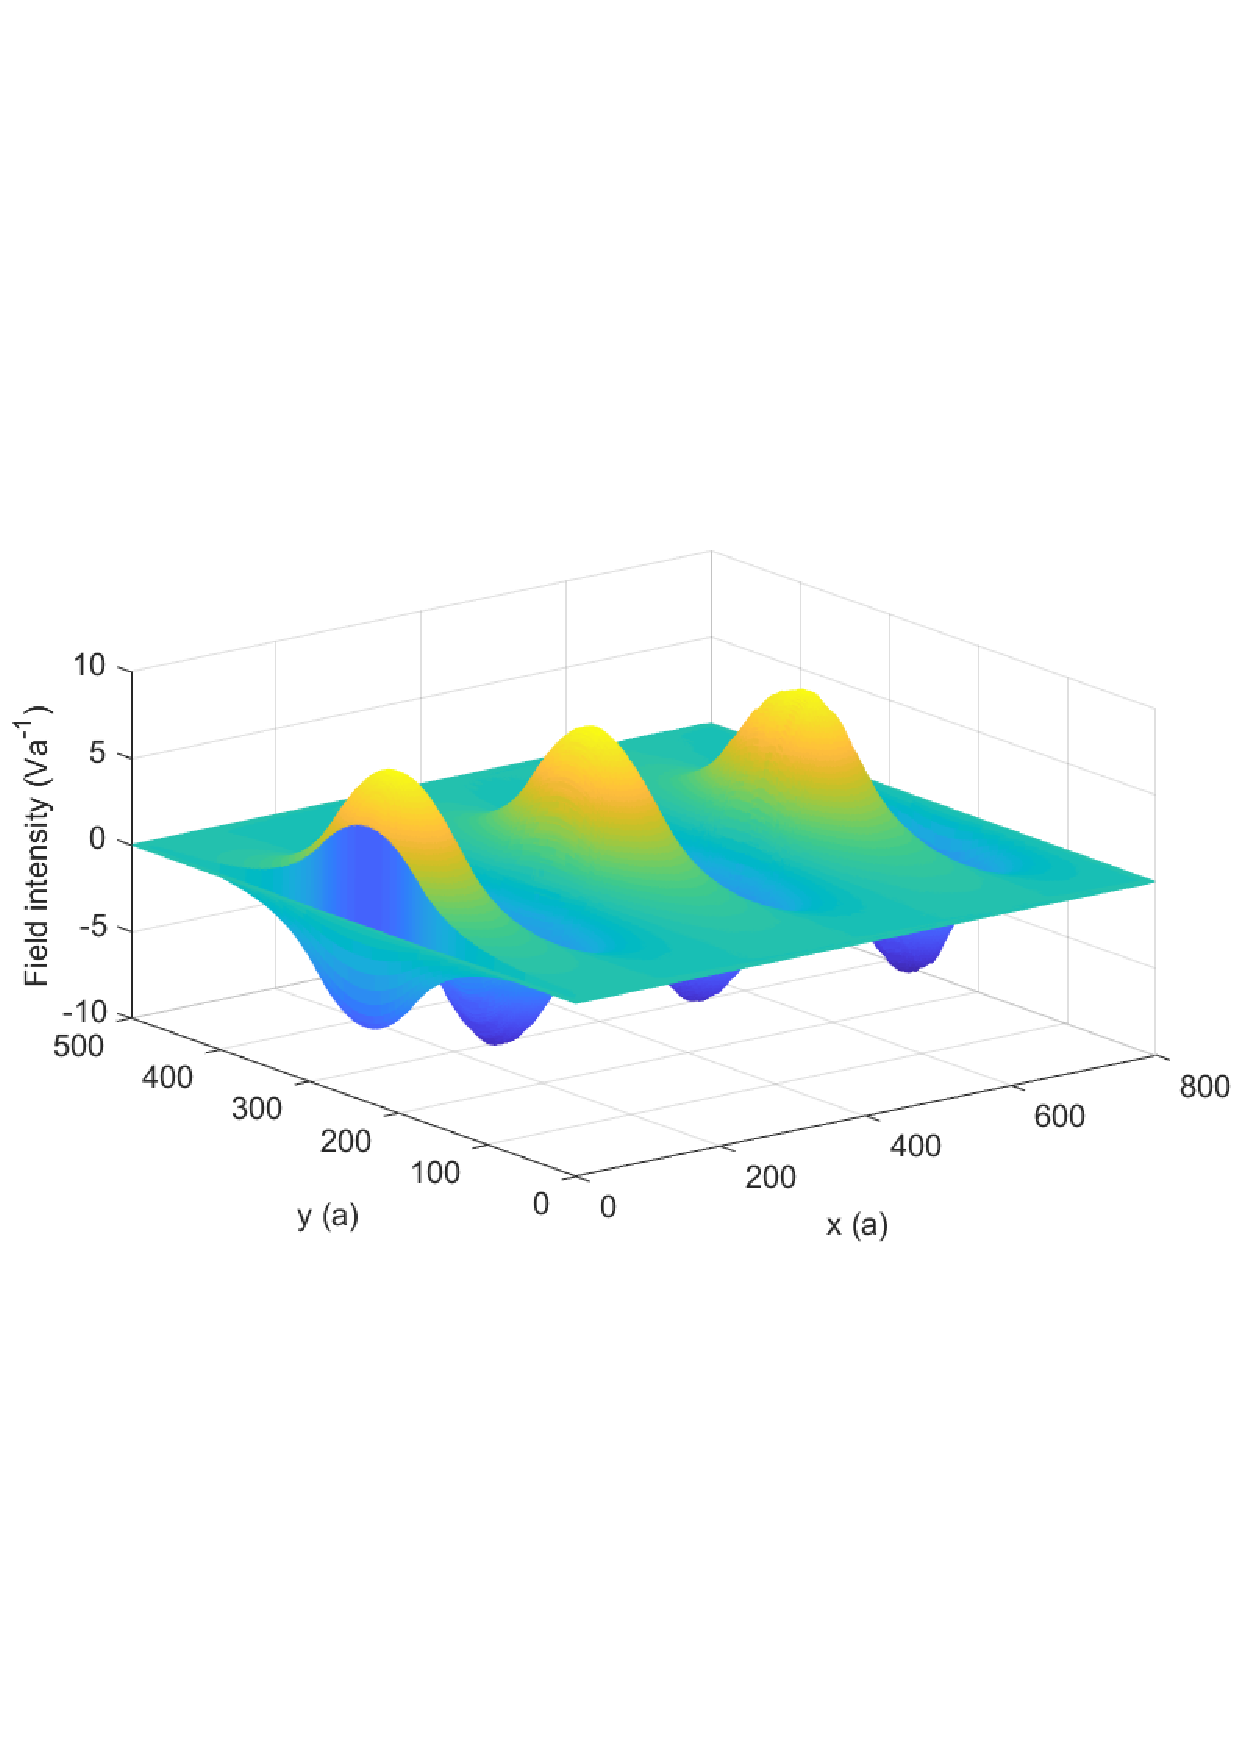
\includegraphics[trim={0 7cm 0 7cm}, scale=0.6]{graphs/modes/untitled.pdf}
	\caption[First two TE modes of a slab dielectric]{$3D$ representation of the electric $E_z$ field profile for mode $\ket{1}$. The excitation of the first fundamental mode is seen at $20 a$. $a$ is a variable length that can be adjusted to scale the entire simulation.}
	\label{fig:3dmode}
\end{figure}


\section{Demonstration of direct photonic transitions}

Here, a direct mode conversion is demonstrated through \textit{FDTD}. The waveguide is chosen to be of length $23 \mu m$ and width $1.1 \mu m$. From the previous band structure calculations, the mode $\ket{1}$ is known to exist at a frequency $\omega_1 = 0.129 (2 \pi c/a)$, and $\ket{2}$ at $\omega_2 = 0.199 (2 \pi c/a)$. Modulation is carried out from ... to ... The spatial discretisation is chosen as $\Delta x = \Delta y = 0.04$. A detector ($D_1$)is placed at $22 \mu m$ to collect the incident field after modulation, and another detector placed in the region between the source and the beginning of modulation($D_2$). To ensure the steady state solution is reached, the simulation is run for $10 000$ time steps. The results are shown in figure \ref{fig:reciprocalmode}. Importantly, we observe perfect mode conversion agreeing with the expected theory. The Fourier transform of the detector outputs illustrates the input $\ket{1}$ mode at $\omega_1 = 0.129 (2\pi c/a)$ and output in mode $\ket{2}$ at $\omega_2 = 0.199 (2\pi c/a)$. Additionally, a weak higher order mode $\ket{3}$ is observed at frequency $\omega_3 = 0.269 (2\pi c/a)$ in the output. The existence of the higher order mode is attributed to a further direct transition of the 2nd mode. 

\begin{figure}[t]
	\centering
	\setlength{\figH}{0.4\textwidth}
	\setlength{\figW}{0.7\textwidth}
	% This file was created by matlab2tikz.
%
%The latest updates can be retrieved from
%  http://www.mathworks.com/matlabcentral/fileexchange/22022-matlab2tikz-matlab2tikz
%where you can also make suggestions and rate matlab2tikz.
%
\definecolor{mycolor1}{rgb}{0.00000,0.44700,0.74100}%
\definecolor{mycolor2}{rgb}{0.85000,0.32500,0.09800}%
%
\begin{tikzpicture}

\begin{axis}[%
width=0.8\figW,
height=0.25\figH,
at={(0\figW,0\figH)},
scale only axis,
xmin=0,
yticklabel style={/pgf/number format/fixed},
xticklabel style={/pgf/number format/fixed},
xmax=0.35,
xlabel={$\omega\text{ (2}\pi\text{c/a)}$},
ymin=0,
ymax=1,
ylabel={Photon flux (n)},
axis background/.style={fill=white}
]
\addplot [color=mode2, line width = 0.2mm]
  table[row sep=crcr]{%
0	6.90869460877597e-05\\
0.117304596739771	0.000462718159760289\\
0.125978998091404	0.000297382378737554\\
0.128180961511434	0.000352644284727033\\
0.132184531366034	0.00136759188320346\\
0.135987922727904	0.000623862971118383\\
0.139057326283097	0.000828198409184244\\
0.141859825181316	0.000660951377172703\\
0.144595597915293	0.000880803909467209\\
0.147264644485026	0.000661010805538709\\
0.149933691054759	0.00104813172839613\\
0.152602737624492	0.000634754192933906\\
0.155471962686955	0.00129608157213545\\
0.158074283092445	0.000596691713695474\\
0.161210412811882	0.00169181178897571\\
0.163679280888885	0.000537857283981813\\
0.165080530337995	0.00187689072933561\\
0.166348327458618	0.00275244484186965\\
0.167349219922268	0.00209827972595544\\
0.169217552521081	0.000402898721760359\\
0.170151718820488	0.00130727836939815\\
0.172286956076274	0.00435614718142729\\
0.173154396211437	0.0034196358130536\\
0.175089454974494	0.00033783528024256\\
0.175823442781171	0.00131201058789543\\
0.178292310858174	0.00759803878669318\\
0.179026298664851	0.0062312771917945\\
0.18102808359215	0.00027904961622327\\
0.18162861907034	0.00151927091309956\\
0.182562785369747	0.0071249763018022\\
0.184097487147343	0.0157152582445836\\
0.18463129646129	0.0151205659351976\\
0.185365284267967	0.0106805311974563\\
0.186966712209806	0.000217090110192109\\
0.18743379535951	0.00173028610106374\\
0.1880343308377	0.0084738673201854\\
0.19043647275046	0.0469296521087703\\
0.19083682973592	0.0445060834473012\\
0.191504091378353	0.0318423586778283\\
0.192972066991706	0.000166588713402138\\
0.193238971648679	0.00213547272719938\\
0.193639328634139	0.0146414049227928\\
0.194306590276573	0.0681609150338081\\
0.195240756575979	0.223097752723171\\
0.197042363010549	0.699960097651519\\
0.198443612459659	0.97368804999049\\
0.198977421773606	1\\
0.199244326430579	0.993817527270956\\
0.199711409580282	0.952638619245898\\
0.200578849715445	0.788690155144477\\
0.204048610256099	0.0333279927147885\\
0.204849324227019	0.000948272372751857\\
0.205049502719749	0.000118381422221425\\
0.205383133540965	0.00313178746896159\\
0.206250573676128	0.0239506141498314\\
0.207384918468265	0.0440519518109421\\
0.207585096960995	0.0445989555779434\\
0.207985453946455	0.0428311430828778\\
0.208652715588888	0.0331925278406733\\
0.210721226680431	0.00079239642971829\\
0.211054857501648	9.47016444752258e-05\\
0.211588666815595	0.00170767127777194\\
0.213790630235625	0.0144060916740212\\
0.214391165713814	0.0130535901147792\\
0.215525510505951	0.00602516654503416\\
0.216726581462331	0.000416984425901878\\
0.217260390776278	0.000189870516005719\\
0.217994378582954	0.0018535808012381\\
0.219729258853281	0.00651767931620006\\
0.220463246659957	0.00597110525495781\\
0.221797769944824	0.00218566643168572\\
0.222932114736961	0.000164174141741524\\
0.223732828707881	0.00057208555282684\\
0.226068244456397	0.00343010723270276\\
0.227069136920047	0.00243806872616137\\
0.22893746951886	0.000187253079213079\\
0.230005088146753	0.000596664568742744\\
0.232006873074053	0.00195118002163341\\
0.233274670194676	0.00126137393949266\\
0.235076276629246	0.00020982260593283\\
0.236610978406843	0.000746757395190256\\
0.238279132512926	0.00113072027948724\\
0.242416154696012	0.000484357236604227\\
0.244618118116042	0.000657299140288004\\
0.248087878656696	0.000384430844256878\\
0.251424186868862	0.000368964292266183\\
0.258296981785925	0.000433298881798105\\
0.261166206848388	0.000634423609358281\\
0.263501622596904	0.000373648648806624\\
0.264569241224798	0.0015449099263416\\
0.265837038345421	0.00477866594844389\\
0.268639537243641	0.0126852117739487\\
0.269440251214561	0.0126759087932213\\
0.270374417513967	0.0109087311214555\\
0.274511439697054	0.000264945650912729\\
0.275779236817677	0.000339848587029845\\
0.277914474073463	0.000734609053077762\\
0.282118222420793	0.000296144777373719\\
0.28465381666204	0.000269904006837685\\
0.287523041724503	0.000192366491871265\\
0.290525719115452	0.000207772302890374\\
0.293461670342159	0.000173096362881653\\
0.296464347733109	0.000200634199863048\\
0.299533751288302	0.000165982888722382\\
0.302669881007738	0.000170916018330081\\
0.305872736891418	0.000176753006553287\\
0.309275771267828	9.51751238431608e-05\\
0.31594838769216	4.70114322019821e-05\\
0.333564095052399	5.21973813545351e-05\\
};
\addlegendentry{$D_2$ (Output)}

\addplot [color=mode1, line width = 0.2mm]
  table[row sep=crcr]{%
0	9.84499576692777e-05\\
0.0667261642433286	0.000428427228356787\\
0.068661223006385	6.13305372691997e-05\\
0.0702626509482249	0.000374831456357638\\
0.0717306265615782	0.000351368916442052\\
0.0734655068319048	0.000123256754796186\\
0.0755340179234478	0.000487187979007375\\
0.0774690766865045	0.000131415964435666\\
0.0794708616138042	0.000583041003948681\\
0.0814059203768609	0.000123277227918717\\
0.0834744314684039	0.000702983462822937\\
0.0853427640672171	0.000109068278802305\\
0.0874780013230037	0.000831396473917945\\
0.0893463339218168	0.000121856262543352\\
0.0914148450133601	0.00105879897365746\\
0.0933499037764167	0.000146538997274126\\
0.0954184148679598	0.00133377399004853\\
0.0973534736310164	0.000164486871907288\\
0.0994219847225595	0.00167874640134524\\
0.101290317321373	0.000160923180471562\\
0.102558114441996	0.00216389097464975\\
0.103292102248673	0.00241524257214309\\
0.105227161011729	0.000129803064990774\\
0.106094601146892	0.00184495690976028\\
0.107095493610542	0.00341718315492523\\
0.107829481417219	0.00230563928595595\\
0.109030552373599	3.30608605381144e-05\\
0.109697814016032	0.00127003609093057\\
0.111099063465142	0.00515347101819752\\
0.111699598943332	0.00401678469918942\\
0.113034122228199	4.04586502038562e-05\\
0.113567931542145	0.00134799796618279\\
0.115102633319742	0.00850395286559102\\
0.115569716469445	0.00743269865808505\\
0.117037692082798	3.74847521795729e-05\\
0.117438049068258	0.00142940397848035\\
0.118172036874935	0.00887593076299287\\
0.119172929338585	0.0165955252138328\\
0.119573286324045	0.0148584893668855\\
0.120507452623451	0.00318449807704857\\
0.120974535773155	3.8371287889083e-05\\
0.121308166594371	0.00168441406063069\\
0.121841975908318	0.0122478495686607\\
0.123309951521671	0.0479045978139261\\
0.123643582342888	0.0439487047529896\\
0.124310843985321	0.0199913970337922\\
0.124978105627754	7.54562746287935e-05\\
0.125178284120484	0.0021059847279834\\
0.125511914941701	0.0202086890353097\\
0.126045724255648	0.0992294441321038\\
0.126913164390811	0.370292542497138\\
0.128848223153867	0.995328829661499\\
0.128981675482354	1\\
0.129115127810841	0.997360946624525\\
0.129448758632057	0.959402049129023\\
0.130116020274491	0.769030373043881\\
0.132451436023007	0.0240565336073533\\
0.132985245336954	4.48384782758549e-05\\
0.133252149993927	0.00335261462704084\\
0.13472012560728	0.0467472013009338\\
0.134987030264254	0.0448349887504631\\
0.135587565742444	0.0297499812744499\\
0.136855362863067	0.000366988704898708\\
0.13732244601277	0.00146520772117942\\
0.138857147790367	0.0163715424299369\\
0.139257504775827	0.0147236468621543\\
0.140992385046153	2.33173488148886e-05\\
0.141459468195857	0.00125620832661566\\
0.14292744380921	0.00815906522325061\\
0.143461253123156	0.00666437845181656\\
0.145062681064996	3.97393674484992e-05\\
0.145663216543186	0.00141873686971694\\
0.146931013663809	0.0049064410312829\\
0.147598275306243	0.0036444960007358\\
0.148999524755353	2.07389463589003e-05\\
0.149666786397786	0.000949168867018013\\
0.151001309682653	0.0033086037718042\\
0.151735297489329	0.00219941722131867\\
0.153003094609952	2.31696749273258e-05\\
0.153803808580872	0.000875541856105944\\
0.155004879537252	0.0022946879878436\\
0.155939045836659	0.00118502317076197\\
0.157006664464552	2.50932747978272e-05\\
0.157940830763959	0.000870234729765329\\
0.159008449391852	0.00175351556770953\\
0.160009341855502	0.000822553119057101\\
0.161076960483395	2.5835821583664e-05\\
0.162278031439775	0.00100985651658969\\
0.163278923903425	0.00127677268050475\\
0.165480887323455	0.000174831306815948\\
0.167282493758025	0.00100268275262039\\
0.169484457178054	0.000154362218679482\\
0.171286063612624	0.000837581992396252\\
0.173554753196898	0.000156493639497102\\
0.175356359631467	0.000664462792619336\\
0.177558323051497	0.000139270865808117\\
0.17942665565031	0.00054846371981343\\
0.181561892906097	0.000129298783461129\\
0.183496951669153	0.000454102606039175\\
0.18563218892494	0.000138974956166438\\
0.187567247687996	0.000371353963459331\\
0.18963575877954	0.000127635902729795\\
0.191770996035326	0.000327556641592119\\
0.193839507126869	0.000284120381486952\\
0.198310160131172	0.00147711410892404\\
0.199511231087552	0.00162237441253588\\
0.202980991628205	0.000349764060434188\\
0.209787060381025	0.000112369158659753\\
0.212189202293785	9.03789330184424e-05\\
0.214658070370788	0.000213182953904933\\
0.256028292201651	4.36960900880301e-05\\
0.264235610403581	1.15791841748258e-05\\
0.272576380933997	7.78270854289165e-05\\
0.27564578448919	0.000118218973406359\\
0.282184948585036	5.81626725664197e-05\\
0.288056851038449	4.09973175865552e-05\\
0.297865597182219	2.1872373606513e-05\\
0.308475057296908	1.79951008263401e-05\\
0.32595731232866	2.24253517078221e-05\\
0.333564095052399	1.44925264395912e-05\\
};
\addlegendentry{$D_1$ (Input)}
\end{axis}
\end{tikzpicture}%
	\caption[The modulated waveguide structure]{LR 12.25 and width 1.1}
	\label{fig:reciprocalmode_fourier}
\end{figure} 

\begin{figure}[t]
	\centering
	\setlength{\figH}{0.1\textwidth}
	\setlength{\figW}{0.8\textwidth}
	% This file was created by matlab2tikz.
%
%The latest updates can be retrieved from
%  http://www.mathworks.com/matlabcentral/fileexchange/22022-matlab2tikz-matlab2tikz
%where you can also make suggestions and rate matlab2tikz.
%
\begin{tikzpicture}

\begin{axis}[%
width=0.8\figW,
height=0.1\figH,
at={(0,0\figH)},
scale only axis,
point meta min=-0.348002718984685,
point meta max=0.348002718984685,
axis on top,
xmin=0,
xmax=23,
xlabel style={font=\color{white!15!black}},
xlabel={$\text{x (}\mu\text{m)}$},
ymin=0,
ymax=5,
ylabel style={font=\color{white!15!black}},
ylabel={$\text{y (}\mu\text{m)}$},
axis background/.style={fill=white},
colormap={mymap}{[1pt] rgb(0pt)=(0,0,1); rgb(31pt)=(1,1,1); rgb(32pt)=(1,1,1); rgb(63pt)=(1,0,0)},
colorbar,
colorbar style={width=.01\linewidth, at={(1.03,0.1\figH)}}
]
\addplot graphics [xmin=0, xmax=23, ymin=0, ymax=5] {graphs/fdtd/reciprocal/LR-1.png};
\draw (0,1.95) -- (23,1.95);
\draw (0,3.05) -- (23,3.05);
\end{axis}
\node[below right]
at (current bounding box.north west) {\textbf{a}};
\end{tikzpicture}%
	\caption[The modulated waveguide structure]{LR 12.25 and width 1.1}
	\label{fig:reciprocalmode}
\end{figure} 

We can further detect the amplitude of each mode while it is undergoing modulation by placing an array of probes in the modulation region ($2 \mu m$ to $21 \mu m$).

\begin{figure}[t]
	\centering
	\setlength{\figH}{0.3\textwidth}
	\setlength{\figW}{0.8\textwidth}
	% This file was created by matlab2tikz.
%
%The latest updates can be retrieved from
%  http://www.mathworks.com/matlabcentral/fileexchange/22022-matlab2tikz-matlab2tikz
%where you can also make suggestions and rate matlab2tikz.
%
\definecolor{mycolor1}{rgb}{0.00000,0.44706,0.74118}%
%
\begin{tikzpicture}

\begin{axis}[%
width=\figW,
height=0.953\figH,
at={(0\figW,0\figH)},
scale only axis,
xmin=0,
xmax=20,
xlabel style={font=\color{white!15!black}},
xlabel={$\text{Modulated length (}\mu\text{ m)}$},
ymin=0,
ymax=1,
ylabel style={font=\color{white!15!black}},
ylabel={Photon flux (n)},
axis background/.style={fill=white},
axis x line*=bottom,
axis y line*=left
]
\addplot [color=mode1, dashed]
  table[row sep=crcr]{%
0.0500000000000007	1\\
0.600000000000001	0.985300295000002\\
0.75	0.978307094000002\\
0.949999999999999	0.966962502000001\\
1.15	0.955967848\\
1.3	0.949529264999999\\
1.5	0.943224780000001\\
1.7	0.936686416000001\\
1.8	0.932249582000001\\
1.9	0.926748569000001\\
2.05	0.916703029000001\\
2.45	0.887680901\\
2.6	0.879206137000001\\
2.75	0.872444712\\
3	0.861921154000001\\
3.1	0.856601853000001\\
3.2	0.850093187999999\\
3.3	0.842329978999999\\
3.45	0.828904319999999\\
3.65	0.810516472\\
3.75	0.802424972000001\\
3.85	0.795547412000001\\
3.95	0.789883003\\
4.15	0.780810902999999\\
4.3	0.773791525\\
4.4	0.767991468000002\\
4.5	0.760904049000001\\
4.6	0.752460313\\
4.75	0.737729229999999\\
5	0.711972104000001\\
5.1	0.703014224\\
5.2	0.69547489\\
5.3	0.689397643\\
5.45	0.68227298\\
5.65	0.672930932\\
5.75	0.666709385000001\\
5.85	0.658846894\\
5.95	0.649328528000002\\
6.1	0.632793121999999\\
6.3	0.610139072999999\\
6.4	0.600146723000002\\
6.5	0.59167617\\
6.6	0.584833270000001\\
6.7	0.579401854\\
7.05	0.562789358\\
7.15	0.555824682000001\\
7.25	0.547066998000002\\
7.35	0.536633309999999\\
7.5	0.519017741999999\\
7.65	0.501544104000001\\
7.75	0.491357915999998\\
7.85	0.482975941999999\\
7.95	0.476501292999998\\
8.05	0.471621516999999\\
8.35	0.459346862\\
8.45	0.453445923\\
8.55	0.445793471000002\\
8.65	0.436371911999998\\
8.75	0.425522733000001\\
9.05	0.391544724999999\\
9.15	0.382366125000001\\
9.25	0.375122797\\
9.35	0.369789205\\
9.5	0.364313612\\
9.7	0.357361956999998\\
9.8	0.352131846999999\\
9.9	0.345060586999999\\
10	0.336144098999998\\
10.15	0.320269456999998\\
10.35	0.298483525000002\\
10.45	0.289129591999998\\
10.55	0.281529978000002\\
10.65	0.275823152000001\\
10.75	0.271776965000001\\
10.95	0.266245011999999\\
11.1	0.261211905\\
11.2	0.256117153000002\\
11.3	0.249257267000001\\
11.4	0.240749382000001\\
11.55	0.226045947999999\\
11.7	0.211409891999999\\
11.8	0.203010402\\
11.9	0.196317837999999\\
12	0.191464149000002\\
12.1	0.1882071\\
12.5	0.178297374\\
12.6	0.173413256\\
12.7	0.167016173\\
12.85	0.155226093\\
13.05	0.138578878000001\\
13.15	0.131404347\\
13.25	0.125685127000001\\
13.35	0.121594976000001\\
13.45	0.118974524999999\\
13.65	0.116139087000001\\
13.8	0.113498306\\
13.9	0.110441199\\
14	0.106067648\\
14.15	0.0973283850000009\\
14.45	0.0778342189999996\\
14.55	0.0727266610000008\\
14.65	0.0688917290000006\\
14.75	0.0663358810000005\\
14.9	0.0643367770000012\\
15.15	0.0620220469999992\\
15.3	0.058759417000001\\
15.45	0.0533310030000003\\
15.9	0.0336135750000004\\
16.05	0.0299902209999985\\
16.2	0.0283199590000009\\
16.65	0.0251553320000006\\
16.8	0.0220658510000007\\
17.3	0.00971707300000091\\
17.45	0.00799669499999922\\
17.65	0.00725801999999831\\
18.05	0.0062111420000015\\
18.95	0.000810164000000668\\
19	0.0007589579999987\\
};
\addlegendentry{$\ket{1}\text{ FDTD}$}

\addplot [color=mode2, dashed]
  table[row sep=crcr]{%
0.0500000000000007	0.00216580500000063\\
0.300000000000001	0.00389339199999839\\
0.800000000000001	0.00923097700000142\\
0.949999999999999	0.0120812470000011\\
1.1	0.0164435689999998\\
1.25	0.0223303679999987\\
1.7	0.0417885349999985\\
1.9	0.047863177\\
2.15	0.0548989800000008\\
2.25	0.0587970210000002\\
2.35	0.0638805620000014\\
2.45	0.0703077289999996\\
2.6	0.0821650920000003\\
2.9	0.107745329\\
3	0.114738200000001\\
3.1	0.120460883\\
3.25	0.127062223999999\\
3.5	0.137206189\\
3.6	0.142823344\\
3.7	0.150052496000001\\
3.8	0.159038304999999\\
3.9	0.169611783000001\\
4.05	0.187336919\\
4.2	0.204989429000001\\
4.3	0.215366144000001\\
4.4	0.223950427999998\\
4.5	0.230592865999999\\
4.6	0.235612417999999\\
4.85	0.246540120999999\\
4.95	0.252889925000002\\
5.05	0.261470484\\
5.15	0.272419852999999\\
5.25	0.285375354999999\\
5.6	0.333812644999998\\
5.7	0.344697831000001\\
5.8	0.353268869000001\\
5.9	0.359647155000001\\
6.05	0.366451613999999\\
6.2	0.373044146000002\\
6.3	0.379229246000001\\
6.4	0.387904595999998\\
6.5	0.399429082000001\\
6.6	0.413532834000002\\
6.75	0.437494039000001\\
6.85	0.453401125999999\\
6.95	0.467697244\\
7.05	0.479428260999999\\
7.15	0.488220944999998\\
7.25	0.494349708000001\\
7.35	0.498636414\\
7.55	0.506436509\\
7.65	0.512325863000001\\
7.75	0.520696685000001\\
7.85	0.531867519999999\\
7.95	0.545624877000002\\
8.05	0.561237255000002\\
8.25	0.593218749999998\\
8.35	0.606909778999999\\
8.4	0.612688882\\
8.45	0.617679139\\
8.5	0.621834007\\
8.6	0.627836250000001\\
8.7	0.631446724\\
8.9	0.636969961999998\\
9	0.64182254\\
9.1	0.649443315999999\\
9.2	0.660075018000001\\
9.3	0.673288244999998\\
9.45	0.695772791\\
9.55	0.710720397999999\\
9.65	0.724234045999999\\
9.75	0.735409001000001\\
9.85	0.743758795000002\\
9.95	0.749293149\\
10.05	0.752544454999999\\
10.3	0.757980238000002\\
10.4	0.762524254999999\\
10.5	0.769885389999999\\
10.6	0.780218057999999\\
10.7	0.792930987999998\\
10.95	0.826663398000001\\
11.05	0.837340602000001\\
11.15	0.845143547999999\\
11.25	0.850075296\\
11.35	0.852711616000001\\
11.7	0.858467137000002\\
11.8	0.863036862000001\\
11.9	0.869857451000001\\
12	0.878796755\\
12.15	0.894789954\\
12.3	0.910713691000002\\
12.4	0.919354812000002\\
12.5	0.925425657000002\\
12.6	0.928702482999999\\
12.7	0.929620229000001\\
13	0.929041353999999\\
13.1	0.931378328000001\\
13.2	0.935854369000001\\
13.3	0.942194992000001\\
13.65	0.967952771\\
13.75	0.973048064\\
13.85	0.976240560000001\\
13.95	0.977506353999999\\
14.05	0.977141171\\
14.4	0.973388779\\
14.5	0.974887964000001\\
14.6	0.978254222\\
14.75	0.985860002999999\\
14.9	0.993843981000001\\
15	0.997743261\\
15.1	0.999751747000001\\
15.2	0.999763796\\
15.3	0.998142525999999\\
15.65	0.989724817999999\\
15.75	0.988928892000001\\
15.85	0.989228392000001\\
16	0.991365311999999\\
16.3	0.996693215000001\\
16.4	0.996914953000001\\
16.5	0.995687951000001\\
16.6	0.992986132999999\\
16.75	0.986996400999999\\
16.9	0.980768823000002\\
17	0.977677851999999\\
17.1	0.975866584999999\\
17.25	0.975143640999999\\
17.45	0.974702435000001\\
17.55	0.973245497000001\\
17.65	0.970560638999999\\
17.8	0.964533818\\
18.25	0.943732929999999\\
18.4	0.938714709999999\\
18.6	0.933800534\\
18.75	0.930079806999998\\
18.85	0.926607670999999\\
18.95	0.921850465999999\\
19	0.918948554\\
};
\addlegendentry{$\ket{2}\text{ FDTD}$}

\addplot [color=mode1]
  table[row sep=crcr]{%
0.0500000000000007	0.999978656\\
0.350000000000001	0.998954493999999\\
0.649999999999999	0.996397148\\
0.949999999999999	0.992314478000001\\
1.25	0.986719026999999\\
1.55	0.979627990000001\\
1.85	0.971063156\\
2.15	0.961050842999999\\
2.45	0.949621816000001\\
2.75	0.936811195000001\\
3.05	0.922658343999998\\
3.4	0.904508496999998\\
3.75	0.884666984999999\\
4.1	0.863216786999999\\
4.45	0.840247606999998\\
4.8	0.815855503000002\\
5.2	0.786367569999999\\
5.6	0.755315596999999\\
6.05	0.718724078000001\\
6.5	0.680620832999999\\
7.05	0.632382093\\
7.7	0.573650849\\
8.8	0.472294262999998\\
9.7	0.390026820999999\\
10.3	0.336730643999999\\
10.8	0.293821841\\
11.25	0.256697761000002\\
11.65	0.225102566\\
12.05	0.195008766000001\\
12.45	0.166580721999999\\
12.8	0.143194922999999\\
13.15	0.121301291000002\\
13.5	0.100991386\\
13.85	0.0823501459999996\\
14.2	0.065455527000001\\
14.5	0.0524183540000003\\
14.8	0.0407565070000011\\
15.1	0.0305058199999984\\
15.4	0.021697790000001\\
15.7	0.0143594839999999\\
16	0.00851344999999881\\
16.3	0.0041776519999992\\
16.6	0.00136541299999848\\
16.9	8.53748000011478e-05\\
17.2	0.000341469999998623\\
17.5	0.00213291200000043\\
17.8	0.00545419599999875\\
18.1	0.0102951160000018\\
18.4	0.016640798000001\\
18.7	0.0244717419999994\\
19	0.0337638849999991\\
};
\addlegendentry{$\ket{1}\text{ Theory}$}

\addplot [color=mode2]
  table[row sep=crcr]{%
0.0500000000000007	2.13440999985437e-05\\
0.350000000000001	0.00104550600000053\\
0.649999999999999	0.00360285200000021\\
0.949999999999999	0.00768552199999917\\
1.25	0.0132809730000005\\
1.55	0.0203720099999991\\
1.85	0.0289368440000004\\
2.15	0.0389491570000011\\
2.45	0.0503781839999995\\
2.75	0.0631888049999993\\
3.05	0.0773416560000015\\
3.4	0.0954915030000016\\
3.75	0.115333015000001\\
4.1	0.136783213000001\\
4.45	0.159752393000002\\
4.8	0.184144496999998\\
5.2	0.213632430000001\\
5.6	0.244684403000001\\
6.05	0.281275921999999\\
6.5	0.319379167000001\\
7.05	0.367617907\\
7.7	0.426349151\\
8.8	0.527705737000002\\
9.7	0.609973179000001\\
10.3	0.663269356000001\\
10.8	0.706178159\\
11.25	0.743302238999998\\
11.65	0.774897434\\
12.05	0.804991233999999\\
12.45	0.833419278000001\\
12.8	0.856805077000001\\
13.15	0.878698709000002\\
13.5	0.899008614\\
13.85	0.917649854\\
14.2	0.934544472999999\\
14.5	0.947581646\\
14.8	0.959243492999999\\
15.1	0.969494180000002\\
15.4	0.978302209999999\\
15.7	0.985640516\\
16	0.991486550000001\\
16.3	0.995822348000001\\
16.6	0.998634587000002\\
16.9	0.999914624999999\\
17.2	0.999658530000001\\
17.5	0.997867088\\
17.8	0.994545804000001\\
18.1	0.989704884000002\\
18.4	0.983359201999999\\
18.7	0.975528258000001\\
19	0.966236115000001\\
};
\addlegendentry{$\ket{2}\text{ Theory}$}

\end{axis}
\end{tikzpicture}%
	\caption[The modulated waveguide structure]{LR 12.25 and width 1.1}
	\label{fig:coherencelength}
\end{figure} 


\begin{figure}[t]
\centering
\setlength{\figH}{1\textwidth}
\setlength{\figW}{1\textwidth}
\begin{tikzpicture}
    \begin{axis}[%
width=0.8\figW,
height=0.1\figH,
at={(0\figW,0\figH)},
scale only axis,
axis on top,
xmin=0,
xmax=23,
xlabel={$\text{x (}\mu\text{m)}$},
ymin=0,
ymax=5,
ylabel={$\text{y (}\mu\text{m)}$},
axis background/.style={fill=white},
]
\fill[fill=eps] (0,1.95) rectangle (23,3.05);
\fill[fill=epsilon] (2,2.5) rectangle (21,3.05);
\fill[fill=modup] (2,2.5) rectangle (21,1.95);
\draw[draw=src, line width=0.5mm] (1,0.8) -- (1,4.2);
\draw[line width=0.5mm, draw=src, ->] (0.5,4.5) -- (1.1,4.5);
\draw[line width=0.5mm, draw=src, ->] (0.5,0.5) -- (1.1,0.5);
%\draw[pattern=north west lines, pattern color=black] (0,0) rectangle (60,0.5);
%\draw[pattern=north west lines, pattern color=black] (0,0) rectangle (0.5,5);
%\draw[pattern=north west lines, pattern color=black] (0,5) rectangle (60,4.5);
%\draw[pattern=north west lines, pattern color=black] (60,0) rectangle (59.5,4.5);
\draw (0,1.95) -- (24.2,1.95) -- (24.2,1.5) -- (35.8,1.5) -- (35.8,1.95) -- (60,1.95);
\draw (0,3.05) -- (24.2,3.05) -- (24.2,3.5) -- (35.8,3.5) -- (35.8,3.05) -- (60,3.05);
\draw[draw=red, dashed, line width=0.7mm] (2,3.05) -- (21,3.05) -- (21,1.95) -- (2,1.95) -- (2,3.05);
\draw[draw=gray, line width = 0.5mm] (1.5,0) -- (1.5,5);
\draw[draw=gray, line width = 0.5mm] (22,0) -- (22,5);
\end{axis}
\end{tikzpicture}
\caption[The modulated waveguide structure]{The modulated waveguide structure. The dark blue region is a material of unity permeability and permittivity of $\epsilon_{wg} = 12.25$. The light blue sections are regions where the permittivity is modulated by an amount $0.1 \epsilon_{wg} \cos(\omega t + \phi)$, with $\phi=0$ on the left and $\phi=\frac{\pi}{2}$ on the right. The modulation region is chosen to only cover the upper half of the waveguide to maximise the coupling. The diagonal lines around the edges represent the \textit{PML} layer, marking the point where the fields effectively decay to zero. Note that the layer width is constant across the \textit{x} and \textit{y} directions. The red line indicates the region over which the modal source is injected, in this case, from left to right (LR).}
\label{fig:cavity}
\end{figure} 

\subsection{Phase-matched non-reciprocal propagation}
width 0.22, eps 12.25

\begin{figure}[t]
	\centering
	\setlength{\figH}{0.4\textwidth}
	\setlength{\figW}{0.7\textwidth}
	% This file was created by matlab2tikz.
%
%The latest updates can be retrieved from
%  http://www.mathworks.com/matlabcentral/fileexchange/22022-matlab2tikz-matlab2tikz
%where you can also make suggestions and rate matlab2tikz.
%
%
\begin{tikzpicture}

\begin{axis}[%
width=0.8\figW,
height=0.4\figH,
at={(0\figW,0\figH)},
scale only axis,
xmin=-3,
xmax=3,
xlabel style={font=\color{white!15!black}},
xlabel={Wavevector $k$ ($2 \pi /a$)},
ymin=0,
ymax=1,
ylabel style={font=\color{white!15!black}},
ylabel={Frequency $\omega$ ($2\pi c/a$)},
axis background/.style={fill=white},
legend pos=south east
]
%\draw[dashed] (-3,0.6468) -- (3,0.6468);
%\draw[dashed] (-3,0.8879) -- (3,0.8879);
%\node at (2.8,0.767) {$\Omega$};
%\draw[dashed] (1.836,0.6468) -- (1.836,0);
%\draw[dashed] (1.367,0.8879) -- (1.367,0);
\draw[->] (1.836,0.6468) -- (1.367,0.8879);
\node[label={90:{$\ket{1}$}},circle,fill=mode1,inner sep=2pt] at (1.836,0.6468) {};
\node[label={90:{$\ket{2}$}},circle,fill=mode2,inner sep=2pt] at (1.367,0.8879) {};
%\node[label={180:{}},circle,fill=mode3,inner sep=2pt] at (-2.305,0.8879) {};
\addplot [color=mode1, forget plot, line width=1.0pt]
table[row sep=crcr]{%
	-0	0\\
	-0.0425483776636622	0.04\\
	-0.112747396858924	0.0920000000000001\\
	-0.138703575229707	0.108\\
	-0.242619225661566	0.16\\
	-0.530251013303014	0.268\\
	-0.68277422737238	0.317\\
	-1.13395473723024	0.451\\
	-1.40367460079584	0.527\\
	-3.00095872332965	0.965\\
};
\addlegendentry{Solver};
\addplot [color=mode1, forget plot, line width=1.0pt]
table[row sep=crcr]{%
	-0	0.649\\
	-0.326077818628705	0.656\\
	-0.605487195406852	0.672\\
	-0.681620546537656	0.68\\
	-0.720361604419702	0.706\\
	-0.780889623877291	0.731\\
	-0.822707823290201	0.745\\
	-0.979328562522052	0.791\\
	-1.40286353275794	0.896\\
	-1.58333534884432	0.938\\
	-1.73350139501897	0.973\\
	-1.85486453299797	1.001\\
};
\addplot [color=mode1, forget plot, line width=1.0pt]
  table[row sep=crcr]{%
0.00856527091199988	0.0089999999999999\\
0.0355740339675572	0.0329999999999999\\
0.0773642883861596	0.0680000000000001\\
0.108965071776361	0.0899999999999999\\
0.216446056096282	0.148\\
0.266469085354788	0.17\\
0.44579687604775	0.239\\
0.779460193245421	0.347\\
0.90346776025157	0.384\\
2.38185947042077	0.796\\
3.00095872332965	0.965\\
};
\addplot [color=mode1, forget plot, line width=1.0pt]
  table[row sep=crcr]{%
0	0.649\\
0.241290268767007	0.653\\
0.432426865263543	0.661\\
0.681620546537656	0.68\\
0.70634705751922	0.698\\
0.812185645324833	0.742\\
0.983207321695099	0.792\\
1.48370503209761	0.915\\
1.85486453299797	1.001\\
};
\addplot [name path=A, color=black, line width=1.0pt]
  table[row sep=crcr]{%
0.00996678000000006	0.00996678000000006\\
1.00664	1.00664\\
};
\addplot [color=mode3, dashed, line width=1.0pt]
  table[row sep=crcr]{%
0.00996678000000006	0.00783098999999998\\
0.149502	0.108661\\
0.199336	0.137065\\
0.259136	0.166038\\
0.33887	0.199306\\
0.448505	0.239874\\
0.598007	0.290189\\
0.797342	0.352394\\
1.07641	0.434535\\
1.48505	0.549875\\
3	0.965172\\
};
\addlegendentry{MPB};
\addplot [color=mode3, dashed, line width=1.0pt, forget plot]
  table[row sep=crcr]{%
0.00996678000000006	0.248465\\
0.0398670999999999	0.251399\\
0.0797342000000001	0.260564\\
0.159468	0.294355\\
0.209302	0.32355\\
0.269103	0.364287\\
0.33887	0.417217\\
0.657807	0.673008\\
0.697674	0.695525\\
0.747508	0.71813\\
0.807309	0.740237\\
0.89701	0.768316\\
1.02658	0.803978\\
1.22591	0.85408\\
1.85382	1.00166\\
};
\addplot [name path=B, line width=1.0pt, color=black]
  table[row sep=crcr]{%
0	0\\
-1.00664	1.00664\\
};

\addplot [color=mode3, dashed, forget plot, line width=1.0pt]
  table[row sep=crcr]{%
-0	0\\
-0.119601	0.0893928000000002\\
-0.199336	0.137065\\
-0.289037	0.179054\\
-0.418605	0.229214\\
-0.61794	0.296612\\
-0.92691	0.391046\\
-1.42525	0.533211\\
-2.51163	0.831749\\
-3	0.965172\\
};
\addplot [color=mode3, dashed, forget plot, line width=1.0pt]
  table[row sep=crcr]{%
-0	0.248268\\
-0.0498339000000001	0.253143\\
-0.0996678	0.267229\\
-0.159468	0.294355\\
-0.229236	0.336534\\
-0.318937	0.401633\\
-0.458472	0.515573\\
-0.627907	0.653101\\
-0.687708	0.690319\\
-0.757475	0.722111\\
-0.857143	0.756346\\
-1.02658	0.803978\\
-1.33555	0.880479\\
-1.85382	1.00166\\
};
\end{axis}



\end{tikzpicture}%
	\caption[]{}
	\label{fig:bandyu}
\end{figure} 

To determine the coherence length, we run the simulation for $15 \mu m$ and calculate the amplitudes of each mode along the length of modulation. Our design proposed here provides a $50 \%$ reduction in device footprint. By modulating each half of the wave guide with a $pi/2$ phase difference, the coherence length can be reduced drastically. To determine the coherence length, the simulation is run for an arbitrarily large modulation region and the amplitude of each mode is calculated at each point in the waveguide,

Our proposed device marks a $50 \%$ size reduction on previous phase matched structures, as the modulated structure is split with a $\pi/2$ phase difference.

LR:
\begin{figure}[t]
	\centering
	\setlength{\figH}{0.4\textwidth}
	\setlength{\figW}{0.8\textwidth}
	\begin{subfigure}[t]{0.5\textwidth}
	% This file was created by matlab2tikz.
%
%The latest updates can be retrieved from
%  http://www.mathworks.com/matlabcentral/fileexchange/22022-matlab2tikz-matlab2tikz
%where you can also make suggestions and rate matlab2tikz.
%
\begin{tikzpicture}

\begin{axis}[%
width=0.35\figW,
height=0.2\figH,
at={(0\figW,0.75\figW)},
scale only axis,
point meta min=-1,
point meta max=1,
axis on top,
clip=false,
xmin=0,
xmax=10,
ymin=0,
ymax=1,
xlabel = {x ($\mu m$)},
ytick={0,0.5,1},
yticklabels={$0$,$0.5$, $1$},
ylabel={$\text{y (}\mu\text{m)}$},
axis background/.style={fill=white},
colormap={mymap}{[1pt] rgb(0pt)=(0,0,1); rgb(31pt)=(1,1,1); rgb(32pt)=(1,1,1); rgb(63pt)=(1,0,0)},
colorbar,
colorbar style={width=.02\linewidth, at={(1.05,0.1\figH)}, anchor=east,ytick={-1,1}},
colorbar style={title={$V / \mu m$}}
]
\addplot graphics [xmin=0, xmax=10, ymin=0, ymax=1] {graphs/fdtd/phasematch/LR/field-1.png};
\node at (-1,2) {\textbf{(a)}};
\node at (2,1.2) {$\ket{1} \rightarrow$};
\node at (8,1.2) {$\rightarrow \ket{2}$};
\end{axis}

\begin{axis}[%
width=0.35\figW,
height=0.2\figH,
at={(0\figW,0.5\figW)},
scale only axis,
point meta min=-1,
point meta max=1,
axis on top,
xmin=0,
clip=false,
xmax=10,
ymin=0,
ymax=1,
xlabel = {x ($\mu m$)},
ytick={0,0.5,1},
yticklabels={$0$,$0.5$, $1$},
ylabel={$\text{y (}\mu\text{m)}$},
axis background/.style={fill=white},
colormap={mymap}{[1pt] rgb(0pt)=(0,0,1); rgb(31pt)=(1,1,1); rgb(32pt)=(1,1,1); rgb(63pt)=(1,0,0)},
colorbar,
colorbar style={width=.02\linewidth, at={(1.05,0.1\figH)}, anchor=east,ytick={-1,1}}
]
\addplot [forget plot] graphics [xmin=0, xmax=10, ymin=0, ymax=1] {graphs/fdtd/phasematch/RL/fieldRL-1.png};
\node at (-1,2) {\textbf{(b)}};
\node at (2,1.2) {$\bra{1} \leftarrow$};
\node at (8,1.2) {$\leftarrow \bra{1}$};
\end{axis}

\begin{axis}[%
width=0.35\figW,
height=0.2\figH,
at={(0\figW,0.25\figW)},
scale only axis,
point meta min=-1,
point meta max=1,
axis on top,
xmin=0,
xmax=10,
ymin=0,
ymax=1,
ytick={0,0.5,1},
clip=false,
xlabel = {x ($\mu m$)},
yticklabels={$0$,$0.5$, $1$},
ylabel={$\text{y (}\mu\text{m)}$},
axis background/.style={fill=white},
colormap={mymap}{[1pt] rgb(0pt)=(0,0,1); rgb(31pt)=(1,1,1); rgb(32pt)=(1,1,1); rgb(63pt)=(1,0,0)},
colorbar,
colorbar style={width=.02\linewidth, at={(1.05,0.1\figH)}, anchor=east,ytick={-1,1}}
]
\addplot [forget plot] graphics [xmin=0, xmax=10, ymin=0, ymax=1] {graphs/fdtd/phasematch/TR/fieldTR-1.png};
\node at (-1,2) {\textbf{(c)}};
\node at (2,1.2) {$\bra{2} \leftarrow$};
\node at (8,1.2) {$\leftarrow \bra{2}$};
\end{axis}
\end{tikzpicture}%
	\end{subfigure}%
	\begin{subfigure}[t]{0.5\textwidth}
	% This file was created by matlab2tikz.
%
%The latest updates can be retrieved from
%  http://www.mathworks.com/matlabcentral/fileexchange/22022-matlab2tikz-matlab2tikz
%where you can also make suggestions and rate matlab2tikz.
%
\begin{tikzpicture}

\begin{axis}[%
width=0.4\figW,
height=0.5\figH,
at={(0\figW,1.2\figH)},
scale only axis,
xmin=0.3,
xmax=1,
xtick={0,0.6468,0.8879,1},
xticklabels={$0$,$0.6468$, $0.8879$,$1$},
ymin=0,
ymax=1,
axis background/.style={fill=white},
legend pos = north west
]
\addplot [color=mode2]
  table[row sep=crcr]{%
0	1.13081867070264e-06\\
0.831674911128847	0.00228169467746064\\
0.838881336867126	0.00202377499498518\\
0.842618002064753	0.0021823789198463\\
0.845820857948432	0.000498850577067556\\
0.849824427803032	0.00520157028131374\\
0.853827997657632	0.000158448678008183\\
0.858365376826178	0.00870591815290878\\
0.862102042023805	5.71739905264046e-05\\
0.865304897907484	0.0133645158166602\\
0.866639421192351	0.0173069295692947\\
0.869041563105111	0.00685264541172503\\
0.870642991046951	5.45500426432088e-05\\
0.872244418988791	0.00968327963340587\\
0.87544727487247	0.048612317596354\\
0.87704870281431	0.0344557748770749\\
0.879183940070097	0.000143863495585039\\
0.88025155869799	0.0162957894625595\\
0.882119891296803	0.170638303761119\\
0.887991793750216	1\\
0.889059412378109	0.94000608315541\\
0.893062982232709	0.255338855812756\\
0.896532742773362	4.8698814648418e-05\\
0.898134170715202	0.0209729769593403\\
0.900269407970989	0.0458723635961076\\
0.902404645226775	0.0252393913145816\\
0.905340596453482	9.65076844801072e-05\\
0.909344166308081	0.0156763040359307\\
0.914148450133601	0.000139489728146369\\
0.918152019988201	0.00780486864007757\\
0.92295630381372	0.000160502704093402\\
0.927226778325293	0.00448871207940704\\
0.932031062150813	0.00033301513591999\\
0.936835345976332	0.00232446948495424\\
0.941639629801852	0.000858887074389303\\
0.946177008970398	0.00117400414562741\\
0.950981292795918	0.00101797533071468\\
0.962458193045771	0.00106641777035499\\
0.969397714127077	0.000883365111032708\\
1.00196008227782	0.000118551983291804\\
1.02357935949266	0.000217825320773857\\
1.05854386955616	0.000104712082806824\\
1.15596406935142	4.98964502413379e-05\\
1.3342563802096	7.9476366254827e-06\\
};
\addlegendentry{$D_2$};
\addplot [color=mode1]
  table[row sep=crcr]{%
0	1.39644351637713e-08\\
0.609076427213103	0.00233545672979218\\
0.616282852951382	0.00430043014561177\\
0.620553327462955	0.000248637961077769\\
0.623756183346635	0.00794154826945515\\
0.626959039230315	7.47971153032267e-05\\
0.630428799770968	0.0162317707623461\\
0.632830941683728	0.00204526366888014\\
0.634699274282541	0.00886138610265252\\
0.637368320852274	0.0457755204955326\\
0.638969748794114	0.0193771513115848\\
0.640037367422007	0.000188198916072357\\
0.641104986049901	0.0271105460388243\\
0.642973318648714	0.289533327408285\\
0.64670998384634	1\\
0.647777602474233	0.934370010222459\\
0.653382600270673	0.00025932622168523\\
0.654717123555539	0.0216863788474451\\
0.656318551497379	0.0470796939868294\\
0.657653074782246	0.0325194712216197\\
0.660055216695006	3.53592225057486e-05\\
0.663258072578686	0.0169734429174946\\
0.666994737776312	8.14290493287295e-05\\
0.669930689003018	0.00862561475450141\\
0.673667354200645	4.6983461483352e-05\\
0.676870210084324	0.00514223972653949\\
0.680606875281951	0.000200359717916987\\
0.683809731165631	0.00342867981165518\\
0.687546396363257	0.000316680510486389\\
0.69101615690391	0.00206216482641941\\
0.69501972675851	0.000905361107496283\\
0.699557105927056	0.000132641242323706\\
0.706496627008362	3.5452938580427e-05\\
0.713436148089669	9.90346817442145e-07\\
0.720642573827948	4.63588478374355e-05\\
0.730251141478987	0.000719353650030063\\
0.741461137071867	0.000186432024472216\\
0.758276130461185	0.000260226636216387\\
0.782297549588784	0.00020597772171671\\
1.3342563802096	1.2617425668715e-06\\
};
\addlegendentry{$D_1$};
\end{axis}

\begin{axis}[%
width=0.4\figW,
height=0.5\figH,
at={(0\figW,0.6\figH)},
scale only axis,
xmin=0.3,
xmax=1,
xtick={0,0.6468,0.8879,1},
xticklabels={$0$,$0.6468$, $0.8879$,$1$},
ymin=0,
ymax=1,
axis background/.style={fill=white},
ylabel={Photon flux $n$}
]
\addplot [color=mode2]
table[row sep=crcr]{%
	0	2.23814667652533e-05\\
	0.599467859562064	0.00433628591280777\\
	0.607208094614289	0.00142683721257098\\
	0.611478569125863	0.00804573548853171\\
	0.616015948294409	2.38495126281268e-05\\
	0.621620946090848	0.0165221829549806\\
	0.626425229916368	0.000103599094986251\\
	0.630695704427941	0.0391146642895677\\
	0.632030227712808	0.0463381738836528\\
	0.634966178939514	0.0150116981517305\\
	0.636567606881354	0.000103582077880748\\
	0.638702844137141	0.0650888340040292\\
	0.64350712796266	0.709716332149051\\
	0.64670998384634	1\\
	0.64831141178818	0.928598166077518\\
	0.657119265468299	5.24822337082398e-05\\
	0.661389739979872	0.0480230679381304\\
	0.665660214491445	0.00758763999999168\\
	0.667528547090259	6.15704802147121e-05\\
	0.672065926258805	0.0163909949062666\\
	0.677937828712218	0.000108656655533057\\
	0.682742112537738	0.00847027912289966\\
	0.688347110334177	9.69307907228156e-05\\
	0.693685203473643	0.00469925536614135\\
	0.699290201270083	0.000427018840210458\\
	0.706763531665336	0.000799353937359193\\
	0.73692375790332	0.000616286557307388\\
	1.04172887616684	6.40938787921375e-05\\
	1.3342563802096	8.46451827918315e-06\\
};
\addplot [color=mode1]
table[row sep=crcr]{%
	0	1.56938971469511e-05\\
	0.601069287503903	0.00451669176492464\\
	0.60800880858521	0.000851375047454139\\
	0.612279283096783	0.00805966375870093\\
	0.617083566922302	9.43746109351995e-05\\
	0.622421660061768	0.0163816251332891\\
	0.626959039230315	4.73278638151164e-05\\
	0.630962609084915	0.0368452763636986\\
	0.632564037026754	0.0462407726858916\\
	0.636834511538327	2.87090439536897e-05\\
	0.638969748794114	0.0661715327694608\\
	0.643774032619634	0.733609777486815\\
	0.64670998384634	1\\
	0.64831141178818	0.926810610112689\\
	0.656852360811326	8.02636681402902e-05\\
	0.661122835322899	0.0475272659011989\\
	0.666727833119339	8.47098536960189e-06\\
	0.671532116944858	0.0167160835620319\\
	0.676870210084324	1.7232287029989e-05\\
	0.681674493909844	0.008387982526882\\
	0.687279491706284	0.000175526652539837\\
	0.692350680188777	0.0048707240118413\\
	0.697688773328243	0.000322623719081649\\
	0.704895199066522	0.000921248344013526\\
	0.73532232996148	0.000254606514388689\\
	0.772955886594717	0.000574892630722301\\
	0.819664201565048	0.000238753269072856\\
	1.06735172323628	5.2218821191552e-06\\
	1.3342563802096	1.2676653494248e-05\\
};
\end{axis}


\begin{axis}[%
width=0.4\figW,
height=0.5\figH,
at={(0\figW,0\figH)},
scale only axis,
xlabel = {Frequency $\omega$ ($2 \pi c/a$)},
xmin=0.3,
xmax=1,
xtick={0,0.6468,0.8879,1},
xticklabels={$0$,$0.6468$, $0.8879$,$1$},
ymin=0,
ymax=1,
axis background/.style={fill=white}
]
\addplot [color=mode2]
table[row sep=crcr]{%
	0	1.22034047884689e-05\\
	0.8311411018149	0.0023013266385894\\
	0.835411576326473	0.00175360932962421\\
	0.839415146181073	0.000965341281125021\\
	0.843685620692646	0.00486553930555145\\
	0.848489904518166	0.000250045011197297\\
	0.853561093000659	0.00825574609007673\\
	0.858098472169205	4.97169960933519e-05\\
	0.861301328052885	0.0109829985996603\\
	0.863436565308671	0.0163494616861442\\
	0.866372516535378	0.00457764465273192\\
	0.867973944477217	1.94703586926526e-05\\
	0.870109181733004	0.013154486929305\\
	0.873578942273657	0.0470453003425026\\
	0.87544727487247	0.0315310399247428\\
	0.87784941678523	2.28975304077395e-05\\
	0.878917035413123	0.0124357545233098\\
	0.880785368011937	0.12400183153239\\
	0.885856556494429	0.869270322219562\\
	0.887991793750216	1\\
	0.889059412378109	0.957556042194106\\
	0.892262268261789	0.513878092808121\\
	0.897600361401255	0.00108842262365672\\
	0.899201789343095	0.0122024441442494\\
	0.902137740569802	0.047153720606177\\
	0.904272977825588	0.0315377211631087\\
	0.908009643023215	1.99441444377335e-05\\
	0.912547022191761	0.0164419581043247\\
	0.916016782732414	0.0041292680012357\\
	0.918152019988201	5.37346492168744e-05\\
	0.92295630381372	0.00824687137239732\\
	0.92856130161016	0.000227034194552944\\
	0.933632490092653	0.00460027207861069\\
	0.938970583232119	0.000392405550539987\\
	0.944308676371585	0.00264766067464928\\
	0.949646769511052	0.000683950981152037\\
	0.954717957993545	0.00165690344143354\\
	0.960056051133011	0.000724562177670807\\
	0.965394144272477	0.000892302126201283\\
	0.97126604672589	0.0010733450416256\\
	0.986212707516396	0.000294720956906636\\
	1.00943341267307	0.000131287278812842\\
	1.02411316880661	0.00048471950436868\\
	1.04066125753895	0.000233818595714919\\
	1.06841934186418	6.61720048844572e-06\\
	1.10391766124163	0.000200101820605481\\
	1.14662240635736	3.20710461947371e-05\\
	1.3342563802096	4.61615482860722e-05\\
};
\end{axis}
\end{tikzpicture}%
	\end{subfigure}
	\caption[]{Phase matched non-reciprocity in a modulated structure. Note that the slight bending at the edges of the simulation are due to the \textit{PML} layer, and do not affect the final solution.}
	\label{fig:bandyu}
\end{figure} 


\begin{figure}[t]
	\centering
	\setlength{\figH}{0.3\textwidth}
	\setlength{\figW}{0.8\textwidth}
	% This file was created by matlab2tikz.
%
%The latest updates can be retrieved from
%  http://www.mathworks.com/matlabcentral/fileexchange/22022-matlab2tikz-matlab2tikz
%where you can also make suggestions and rate matlab2tikz.
%
\definecolor{mycolor1}{rgb}{0.00000,0.44700,0.74100}%
\definecolor{mycolor2}{rgb}{0.85000,0.32500,0.09800}%
\definecolor{mycolor3}{rgb}{0.92900,0.69400,0.12500}%
\definecolor{mycolor4}{rgb}{0.49400,0.18400,0.55600}%
%
\begin{tikzpicture}

\begin{axis}[%
width=0.4\figW,
height=0.5\figH,
at={(0\figW,0\figH)},
scale only axis,
xmin=0,
xmax=5,
ymin=0,
ymax=1,
xlabel = {Modulated length ($\mu m$)},
ylabel = {Photon flux ($n$)},
axis background/.style={fill=white},
axis x line*=bottom,
axis y line*=left
]
\addplot [color=mode1]
  table[row sep=crcr]{%
0.00999999999999979	1\\
0.13	0.992\\
0.2	0.988\\
0.29	0.975\\
0.35	0.967\\
0.55	0.943\\
0.7	0.917\\
0.77	0.906\\
1.08	0.84\\
1.15	0.823\\
1.31	0.787\\
1.49	0.737\\
1.58	0.715\\
2.86	0.335\\
2.93	0.317\\
3.07	0.279\\
3.15	0.259\\
3.26	0.23\\
3.39	0.2\\
3.44	0.189\\
3.59	0.155\\
3.64	0.144\\
3.9	0.0961999999999996\\
4.11	0.0646000000000004\\
4.35	0.0351999999999997\\
4.59	0.0152999999999999\\
4.8	0.00460999999999956\\
5.01	0.00107000000000035\\
};
\addplot [color=mode2]
  table[row sep=crcr]{%
0.00999999999999979	0.00076699999999974\\
0.17	0.00628000000000029\\
0.49	0.0303000000000004\\
0.66	0.0549999999999997\\
0.8	0.0716000000000001\\
0.9	0.0978000000000003\\
0.96	0.113\\
1.05	0.127\\
1.13	0.139\\
1.19	0.155\\
1.25	0.177\\
1.32	0.202\\
1.55	0.251\\
1.73	0.32\\
1.81	0.332\\
1.86	0.341\\
1.92	0.363\\
1.96	0.382\\
2.01	0.408\\
2.09	0.436\\
2.15	0.445\\
2.19	0.449\\
2.26	0.467\\
2.31	0.491\\
2.43	0.549\\
2.51	0.561\\
2.6	0.573\\
2.65	0.592\\
2.81	0.668\\
2.92	0.675\\
2.95	0.678\\
2.99	0.689\\
3.04	0.712\\
3.12	0.756\\
3.17	0.773\\
3.24	0.776\\
3.3	0.774\\
3.35	0.783\\
3.42	0.815\\
3.48	0.847\\
3.53	0.863\\
3.58	0.865\\
3.69	0.858\\
3.72	0.864\\
3.76	0.879\\
3.86	0.926\\
3.9	0.935000000000001\\
3.96	0.931\\
4.05	0.917\\
4.09	0.921\\
4.14	0.939\\
4.21	0.97\\
4.24	0.978\\
4.27	0.981\\
4.3	0.978\\
4.36	0.962\\
4.41	0.951\\
4.45	0.951\\
4.5	0.965\\
4.54	0.981\\
4.59	0.997\\
4.64	0.999\\
4.7	0.983\\
4.77	0.959\\
4.81	0.955\\
4.84	0.958\\
4.88	0.969\\
4.93	0.985\\
4.96	0.991\\
4.99	0.991\\
5.01	0.988\\
};
\addplot [color=mode1, dashed]
  table[row sep=crcr]{%
0.00999999999999979	0.999990209\\
0.22	0.99526858\\
0.43	0.982005207\\
0.64	0.96042884\\
0.86	0.929316078\\
1.09	0.888113089\\
1.33	0.836575682\\
1.6	0.769602103\\
1.9	0.686271286\\
2.29	0.568622403\\
3.2	0.290741175\\
3.51	0.207120884\\
3.78	0.143143349\\
4.02	0.094757081\\
4.25	0.0569368749999999\\
4.47	0.0293268749999998\\
4.68	0.0112758949999998\\
4.89	0.00165378700000041\\
5.01	9.7910900000997e-06\\
};
\addplot [color=mode2, dashed]
  table[row sep=crcr]{%
0.00999999999999979	9.7910900000997e-06\\
0.22	0.00473141999999971\\
0.43	0.0179947929999997\\
0.64	0.0395711600000004\\
0.86	0.0706839219999997\\
1.09	0.111886911\\
1.33	0.163424318\\
1.6	0.230397897\\
1.9	0.313728714\\
2.29	0.431377597\\
3.2	0.709258825\\
3.51	0.792879116\\
3.78	0.856856651\\
4.02	0.905242919\\
4.25	0.943063125\\
4.47	0.970673125\\
4.68	0.988724105\\
4.89	0.998346213\\
5.01	0.999990209\\
};
\end{axis}
\end{tikzpicture}%
	\caption[The modulated waveguide structure]{LR 12.25 and width 1.1}
	\label{fig:coherencelength}
\end{figure} 

\begin{table}[]
	\centering
	\caption[Mode conversions in a phase-matched structure]{Summary of mode conversions in the phase-matched structure}
	\label{my-label}
	\begin{tabular}{|l|l|}
		\hline 
		Direction & Transition \\ \hline
		LR        & $\ket{1} \rightarrow \ket{2}$           \\
		RL        & $\ket{1} \rightarrow \ket{1}$           \\
		TR        & $\ket{2} \rightarrow \ket{2}$          \\ \hline
	\end{tabular}
\end{table}

\section{Motivation for development of frequency domain solutions}
	
Simulating effective modulations of wave-guide structures is evidently a computationally intensive process. Consider the simplest example, a slab waveguide whose permittivity modulation frequency is tuned to stimulate a photonic transition between the first fundamental () and the second odd mode. This requires the modulation frequency to be (), several orders of magnitude lower than the input wave. Since a time-domain simulation requires the time-step to be chosen based on the highest frequency present in the simulation, the massive gap between the optical source frequency and the modulation frequency lead to slow convergence times. This is because the input wave must pass through at minimum one cycle of the modulation. There are however, several benefits granted by the harmonic nature of the modulation. The first is that the modulation generates sidebands at \textit{known} frequencies,
\begin{equation}
\omega_n = \omega_0 \pm n \Omega
\end{equation}
where $\Omega$ is the modulation frequency and $n$ is the set of integers. This is incredibly advantageous: we know in advance every possible frequency that can exist in the simulation space. The second benefit granted is that the modulation is harmonic in nature, and it is this harmonicity that allows for a method of expressing the time dependent modulations in frequency space. Thus, we look towards a modified form of the finite-difference frequency domain where instead of discretising \textit{time} we discretise \textit{frequency} instead.


\begin{table}[]
\centering
\begin{tabular}{|l|l|l|}
\hline
                             & \textit{Time domain}    & \textit{Frequency domain}         \\ \hline
\textit{Memory usage}        & Medium                  & High                              \\ \hline
\textit{Adjacent eigenmodes} & Mixed in final solution & Naturally separated               \\ \hline
\textit{Standard run-time}   & Days                    & Hours                             \\ \hline
\textit{Parallelisation}   & Trivial                 & Non-trivial \\ \hline
\textit{Extension to 3D}   & Trivial                 & Trivial \\ \hline
\end{tabular}
\caption[Comparison of \textit{FDTD} and \textit{FDFD} methods]{Comparison of basic extraction methods and computational expenditure for general finite difference simulations in the time and frequency domain. In this case, parallelisation refers to the property of being able to split the simulation into multiple `chunks' that can be run simultaneously on high-performance clusters.}
\label{comparisonFD}
\end{table}

In table \ref{comparisonFD} the main properties of the time and frequency domain methods are compared.


